% Chapter 5: Single-Model Performance  (FOCUS 1)

\chapter{Single-Model Performance}\label{ch:single-model}



This chapter evaluates the models that downscale one variable at a time. Every result is reported under the two regimes of \sref{subsec:meth-cv}: the CV holdout, where each day of 2020--2023 is predicted by the holdout fold, as well as the unseen year 2024, predicted by the five-fold ensemble. The temperature models are reported first: seven configurations are compared under both regimes, the feature-importance study explains what separates them, and the remainder of the section investigates the selected model in depth. The results of precipitation models follow in \sref{sec:single-precipitation}.



\section{Temperature Model}\label{sec:single-temperature}



\subsection{Model Variants}\label{subsec:single-tmax-variants}



\tref{tab:single-tmax-variants} lists the seven training runs behind all temperature results, with the model names used in every figure and table that follows.



\begin{table}[htbp]

\centering

\caption[The seven temperature runs]{The seven temperature runs. All share the architecture of \sref{sec:meth-architecture} and the setup of \tref{tab:meth-training-setup}; the two \texttt{-clip60} retrains (\texttt{atm-clip60}, \texttt{atm+wind-clip60}) with double the epoch budget and patience and add a gradient clip. Channel counts include the scaffold.}

\label{tab:single-tmax-variants}

\footnotesize

\begin{tabular}{|p{2.9cm}|p{6.4cm}|p{1.2cm}|p{1.2cm}|}

\hline

\textbf{Model name} & \textbf{Context input} & \textbf{Chan.} & \textbf{Epochs} \\

\hline

\texttt{sfc} & ERA5-Land daily-maximum $2\,\mathrm{m}$ temperature, plus the full scaffold & 6 & 30 \\

\hline

\texttt{sfc-nogeo} & as \texttt{sfc}, without the coarse-elevation channel & 5 & 30 \\

\hline

\texttt{atm} & ERA5 pressure-level $z$, $t$, $q$ on six levels at five sampling hours, plus scaffold & 95 & 30 \\

\hline

\texttt{atm+wind} & as \texttt{atm}, with the wind components $u$ and $v$ added & 155 & 30 \\

\hline

\texttt{atm+sfcanchors} & as \texttt{atm}, with ERA5 single-level $2\,\mathrm{m}$ temperature and total precipitation at the five hours appended & 105 & 30 \\

\hline

\texttt{atm-clip60} & as \texttt{atm}; $60$ epochs, patience $20$, gradient clip & 95 & 60 \\

\hline

\texttt{atm+wind-clip60} & as \texttt{atm+wind}; same extended budget & 155 & 60 \\

\hline

\end{tabular}

\end{table}



\subsection{Accuracy, Skill and Generalisation}\label{subsec:single-tmax-headline}



Skill is the CRPSS of \eref{eq:crpss} against the bilinear ERA5-Land reference, which is identical for every model; \tref{tab:single-tmax-headline} lists all individual numerical values for all runs. Every configuration beats the ERA5-Land reference by a wide margin: MAE falls by $1.0$ to $1.5\,^{\circ}\mathrm{C}$ and CRPS by $1.4$ to $1.8\,^{\circ}\mathrm{C}$, the atmospheric models performing better than the  surface models.

\begin{table}[H]
\centering
\caption[Temperature metrics, CV holdout vs 2024 holdout]{Headline metrics of the seven temperature runs of \sref{sec:single-temperature} under the CV holdout (2020--2023) and the 2024 holdout. All values in $^{\circ}\mathrm{C}$ except skill. Every column is comparable across the seven models: MAE, RMSE and CRPS are measured against the fixed MeteoSwiss truth, and skill, the only baseline-relative column,  is scored against ERA5-Land. Green shades the best and red the worst model in each column. The last row is the shared bilinear ERA5-Land reference: it is deterministic, so its CRPS equals its MAE and its skill is zero by definition.}
\label{tab:single-tmax-headline}
\footnotesize
\begin{tabular}{|p{3cm}|p{0.85cm}|p{0.85cm}|p{0.85cm}|p{0.85cm}|p{0.85cm}|p{0.85cm}|p{0.85cm}|p{0.85cm}|}
\hline
& \multicolumn{2}{c|}{\textbf{MAE}} & \multicolumn{2}{c|}{\textbf{RMSE}} & \multicolumn{2}{c|}{\textbf{CRPS}} & \multicolumn{2}{c|}{\textbf{Skill}} \\
\hline
\textbf{Model} & CV & 2024 & CV & 2024 & CV & 2024 & CV & 2024 \\
\hline
\texttt{atm} & 1.24 & 1.21 & 1.65 & 1.66 & 0.92 & 0.91 & 0.641 & 0.642 \\
\hline
\texttt{atm-clip60} & 1.09 & 1.05 & 1.46 & 1.42 & 0.79 & 0.76 & 0.693 & 0.702 \\
\hline
\texttt{atm+wind} & 1.31 & 1.25 & 1.73 & 1.71 & 0.96 & 0.94 & 0.625 & 0.632 \\
\hline
\rowcolor{green!12}\texttt{atm+wind-clip60} & 1.05 & 1.03 & 1.41 & 1.39 & 0.76 & 0.74 & 0.702 & 0.708 \\
\hline
\texttt{atm+sfcanchors} & 1.20 & 1.17 & 1.61 & 1.62 & 0.90 & 0.89 & 0.650 & 0.650 \\
\hline
\texttt{sfc} & 1.42 & 1.47 & 1.87 & 1.97 & 1.03 & 1.08 & 0.597 & 0.576 \\
\hline
\rowcolor{red!12}\texttt{sfc-nogeo} & 1.45 & 1.49 & 1.90 & 1.98 & 1.06 & 1.09 & 0.588 & 0.571 \\
\hline
bilinear ERA5-Land & 2.56 & 2.54 & 3.36 & 3.35 & 2.56 & 2.54 & 0 & 0 \\
\hline
\end{tabular}
\end{table}




Generalisation is strong: the best models achieve a CRPS as low as $0.74\,^{\circ}\mathrm{C}$ on the unseen year. The atmospheric models outperform the surface models on every metric (\fref{fig:single-tmax-slope}), and the gap holds on the year no fold saw. Furthermore they have potential for further improvement with an extended training budget, as evidenced by the performance of the \texttt{atm-clip60} and \texttt{atm+wind-clip60} models. The wind channels need the longer budget before they pay off: at $30$ epochs \texttt{atm+wind} ($155$ channels) is worse than \texttt{atm} ($95$), $1.31$ against $1.24\,^{\circ}\mathrm{C}$ CV MAE, while under the extended budget \texttt{atm+wind-clip60} becomes the best model of the comparison, ahead of \texttt{atm-clip60} at $1.05$ against $1.09$. The training curves show why, and show that the extended run was still improving when it ended (\sref{sec:app-tmax-metrics}). All models with atmospheric input show better generalisation than those limited to surface input.

Including surface anchors improves the performance of the atmospheric model, however the gain is small.



\begin{figure}[H]

\centering

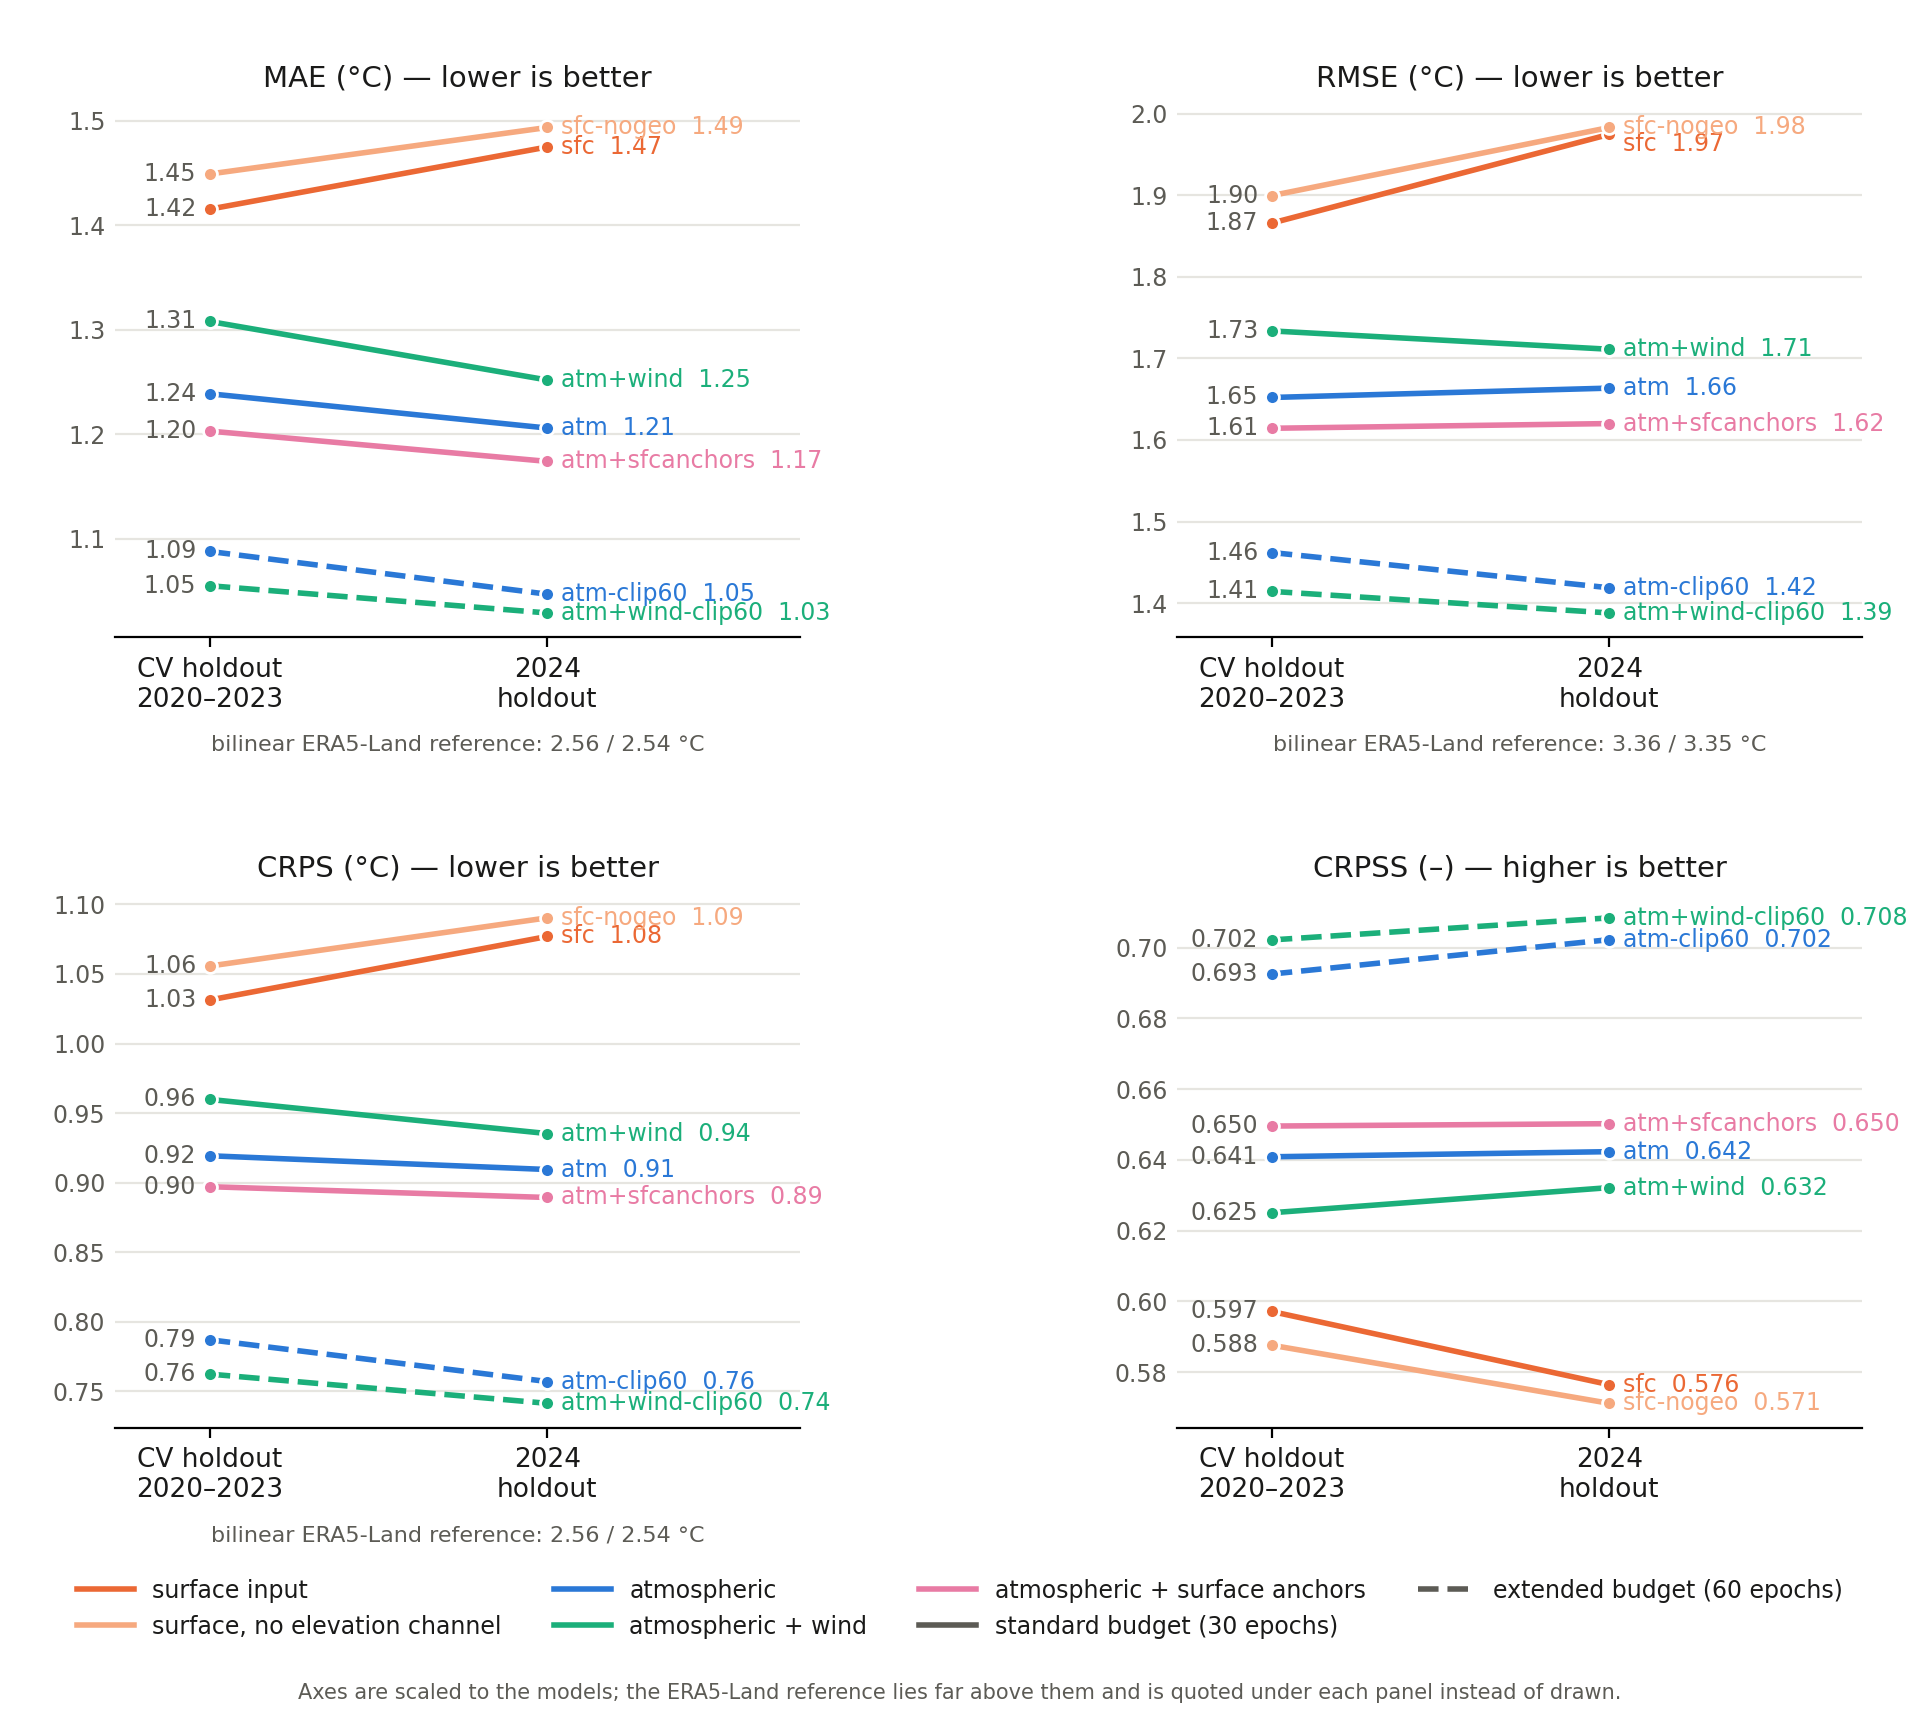
\includegraphics[width=\textwidth]{images/tmax_regime_slope.png}

\caption[Headline metrics from the CV span to 2024]{The four headline metrics of the seven temperature models. Colour encodes the input family, dashed lines the extended-budget retrains. It is clearly visible that the atmospheric input models perform well and generalise well. The surface models lag behind and the generalisation is worse than the CV.}

\label{fig:single-tmax-slope}

\end{figure}







\subsection{Feature Importance}\label{subsec:single-tmax-fi}

For the feature-importance study on temperature we first have a look at the grouped importance for the two input families atmospheric input and surface input. As an additional reference we consider the atmospheric input with the surface anchors. While the surface anchors include the diurnal cycle they are the closest match to the surface input while still being part of the atmospheric input family. All results are evaluated on the 2024 holdout year.





\begin{figure}[H]

\centering

\subfloat[\texttt{sfc}]{%

  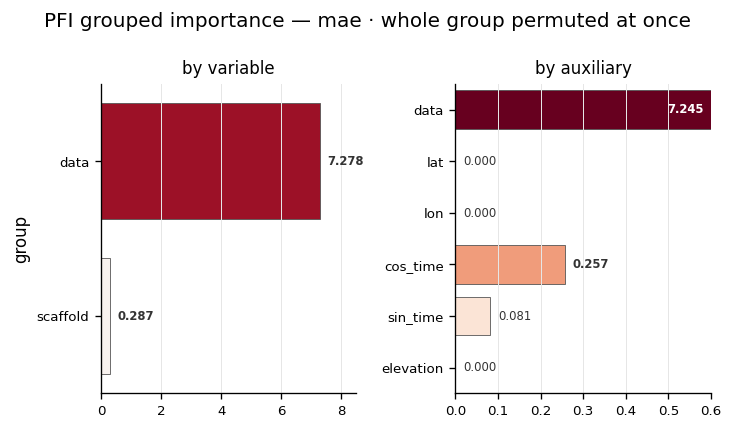
\includegraphics[height=0.285\textwidth]{images/results/tmax__pfi_groups_mae__feature_importance_2024__baseline.png}}\\[2ex]

\subfloat[\texttt{atm}]{%

  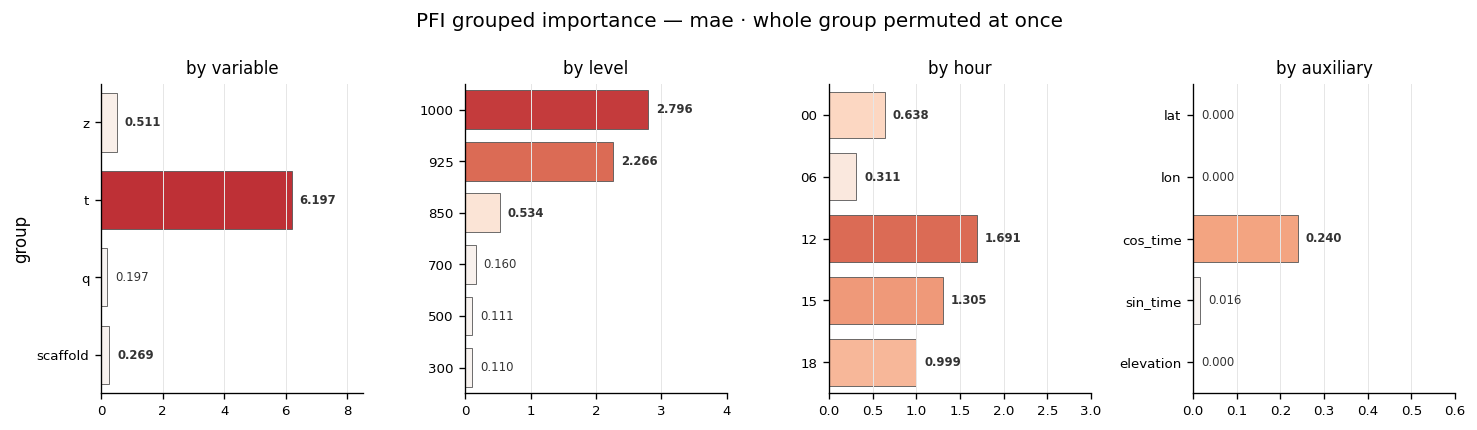
\includegraphics[height=0.285\textwidth]{images/results/tmax__pfi_groups_mae__feature_importance_2024__clean_solo.png}}\\[2ex]

\subfloat[\texttt{atm+sfcanchors}]{%

  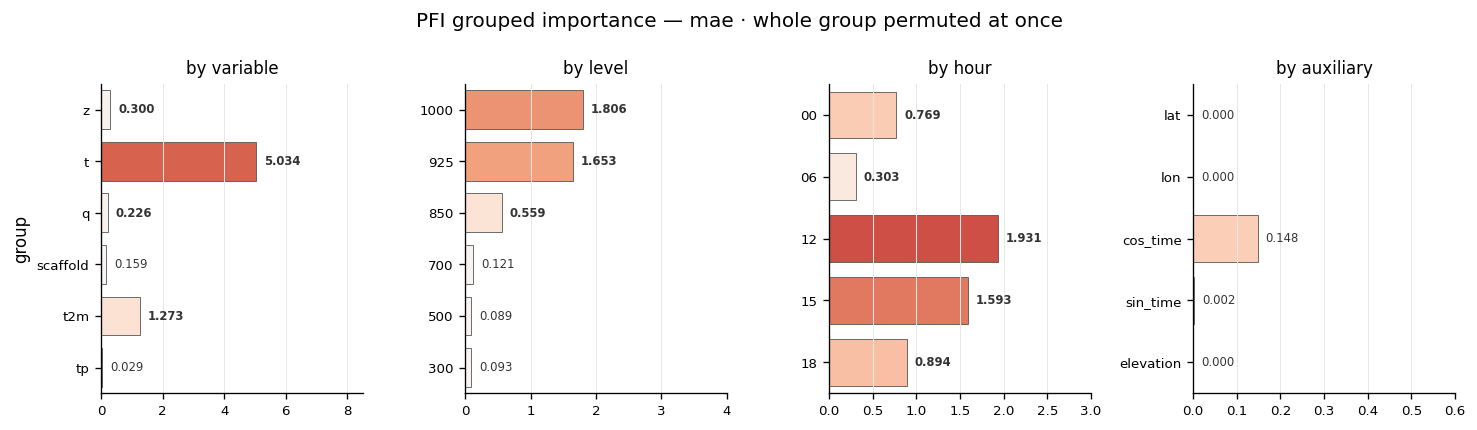
\includegraphics[height=0.285\textwidth]{images/results/tmax__pfi_groups_mae__feature_importance_2024__sfc_anchors.png}}

\caption[Grouped permutation importance across the three input families]{Grouped permutation importance (\sref{subsec:meth-fi-groups}) for the three $30$-epoch input families: the MAE degradation in $^{\circ}\mathrm{C}$ when a whole group is permuted at once. All three models are dominated by close to surface temperature; for the surface model, the seasonal encoding is the only other group with visible impact. The atmospheric input models also show a significant importance of the diurnal cycle information. Even though low altitude pressure levels  in the second half of the day dominate the importance, the higher levels and even night time snapshots still contribute in a non negligible way.}

\label{fig:single-tmax-fi-groups}

\end{figure}
 \fref{fig:single-tmax-fi-groups} presents a good overview to compare the reliance of the different input families. The surface model (a) has only one data source, its data channel carries $7.3\,^{\circ}\mathrm{C}$ of importance, with the seasonal encoding ($0.26$ for its stronger channel) the only other visible input with impact. The remaining scaffold channels score exactly zero, this is by design as a time-invariant channel is unchanged by a permutation along the day axis (\sref{subsec:app-fi-limits}). The atmospheric model (b) spreads a similar importance across its temperature group ($6.2\,^{\circ}\mathrm{C}$), concentrated at $1000$ and $925\,\mathrm{hPa}$ and in the midday and afternoon hours, while geopotential and humidity contribute little but not nothing. With the anchors added (c) the pattern persists, but the $2\,\mathrm{m}$ anchor takes a substantial share ($1.3\,^{\circ}\mathrm{C}$, against $5.0$ for the temperature group) while the precipitation anchor is ignored, and the seasonal encoding falls to its smallest value of the three ($0.15$). The same grouped view for the four remaining configurations is in \sref{sec:app-fi}. The surface anchors are therefore not a substitute for the atmospheric input, but they do provide a small additional signal that the model can use.







Temperature is a relatively easy variable to downscale, so it is not surprising that the surface input model is able to achieve a good performance with only one temperature channel. What remains to be observed here is that the atmospheric input model while missing any meteorological surface input is able to achieve better performance than the surface input model. Therefore we can conclude that the atmospheric input contains more information than the surface input and that the model is able to extract and learn this information. Adding surface anchors gains a slight advantage over the atmospheric input model, but the feature importance study shows that the model still relies on the atmospheric input and does not overwrite the learned information with the surface anchors. 



\subsection{The Downscaled Field}\label{subsec:single-tmax-field}

Before turning to the error statistics we look at the spatial patterns of the modelled fields. \fref{fig:single-tmax-spatial} shows snapshots of the downscaled field. The coarse input resolves the domain into a handful of smooth patches; along the section we have significant alpine topography and cross the Main alpine divide. The reference model does not resolve the terrain details; both downscaling models return the valley-and-ridge swing of the ground-truth reference.

\begin{figure}[htbp]

\centering

\subfloat[A typical day: 25 January 2024, the median-error day with the widest observed range]{%

  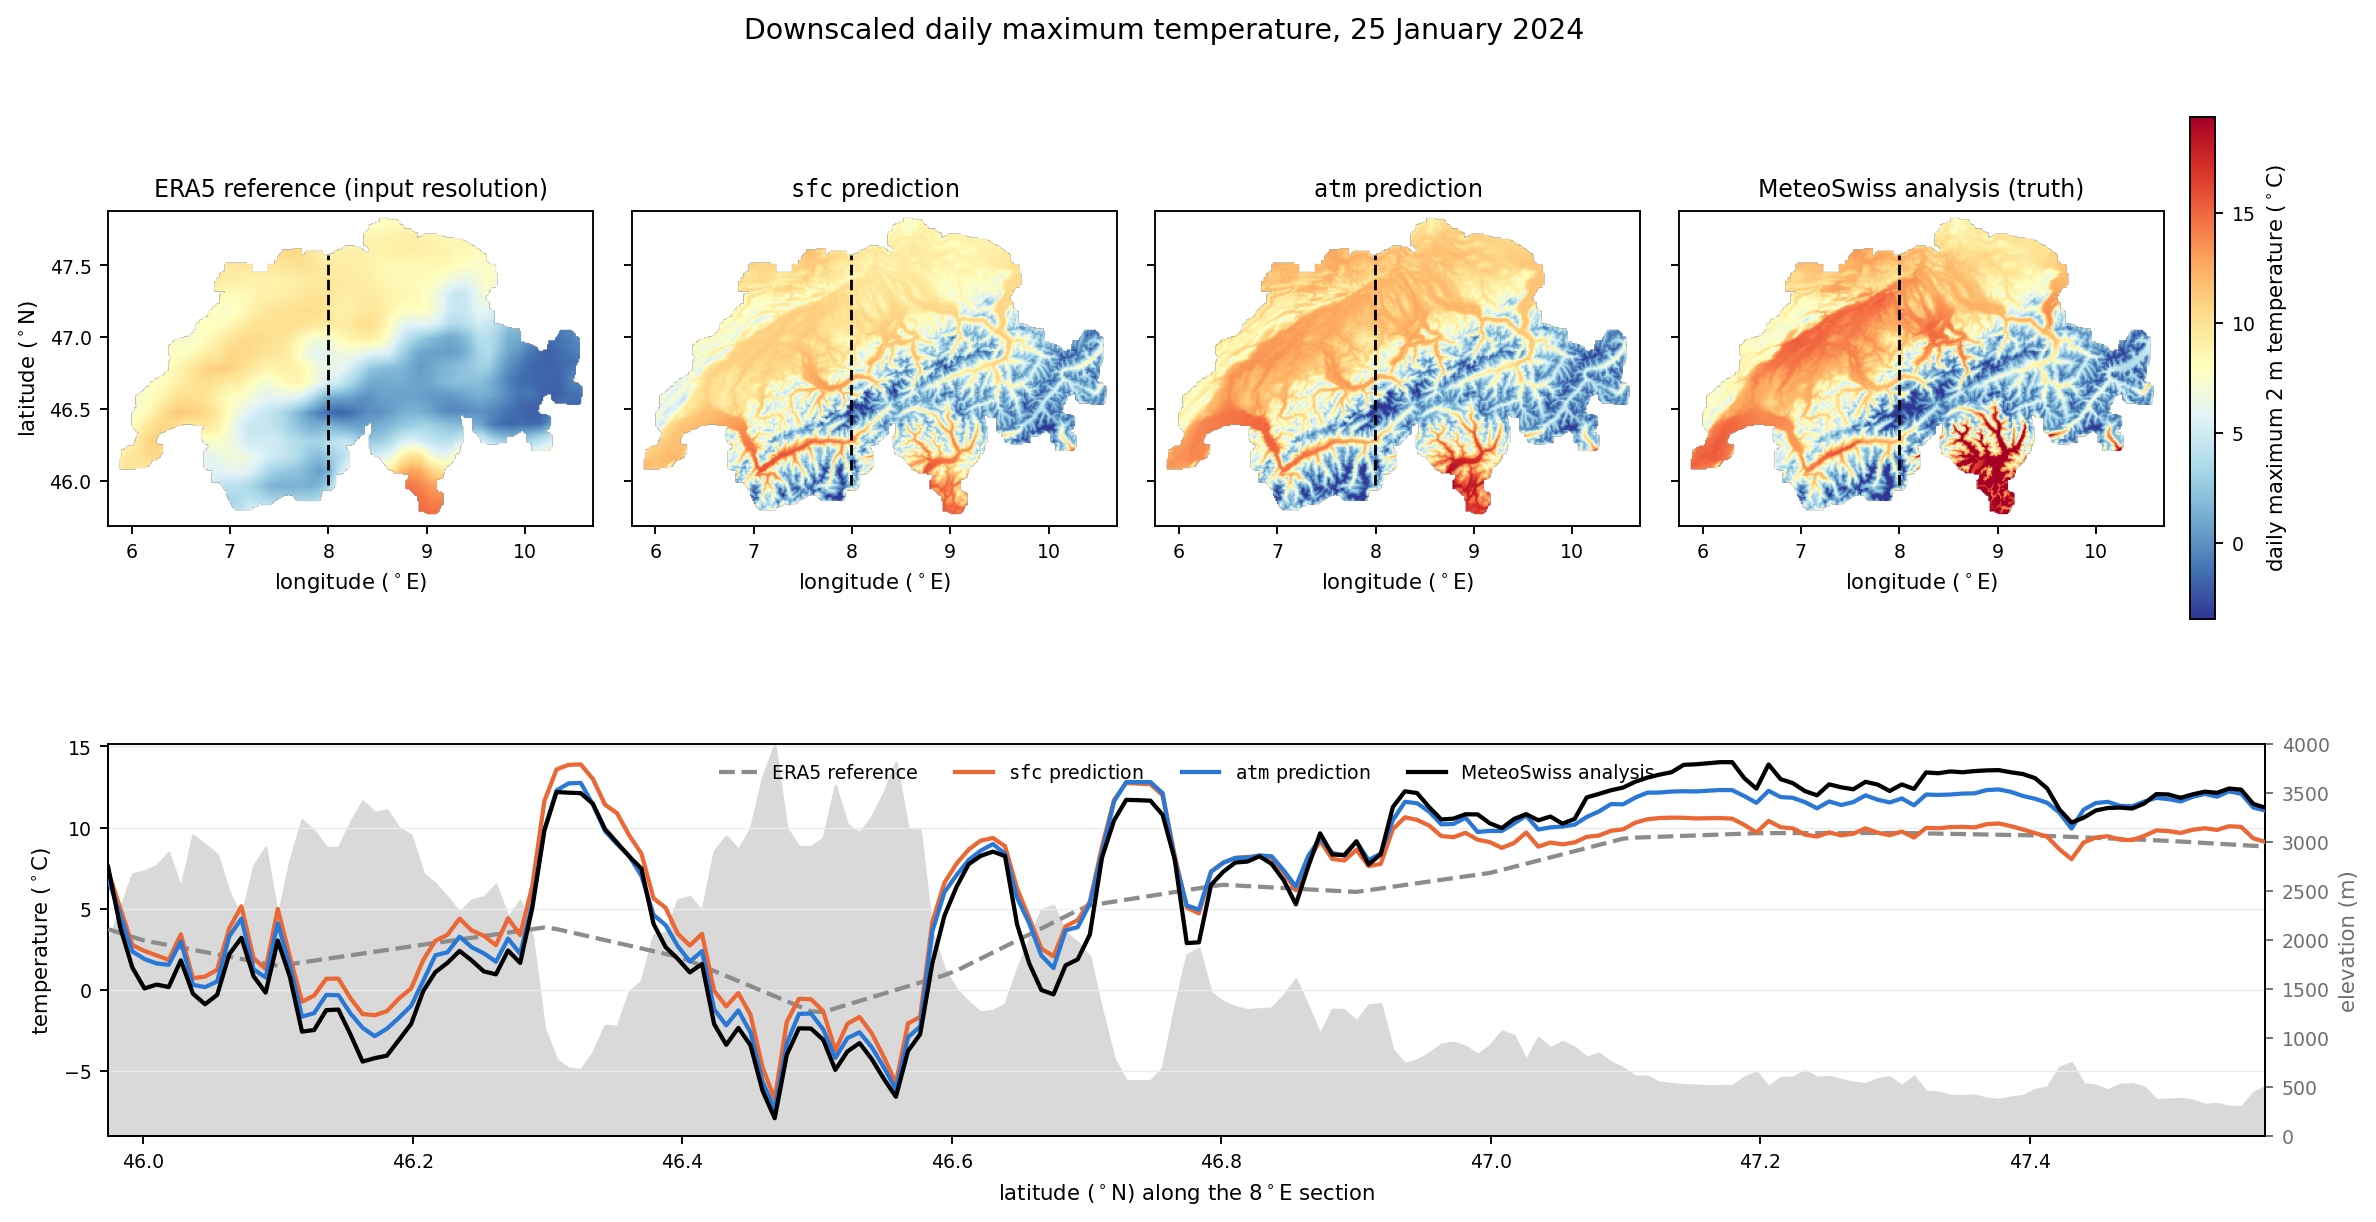
\includegraphics[width=0.74\textwidth]{images/tmax_spatial_section.png}}\\[1ex]

\subfloat[The extreme warm day: 30 July 2024, the highest observed domain-mean maximum]{%

  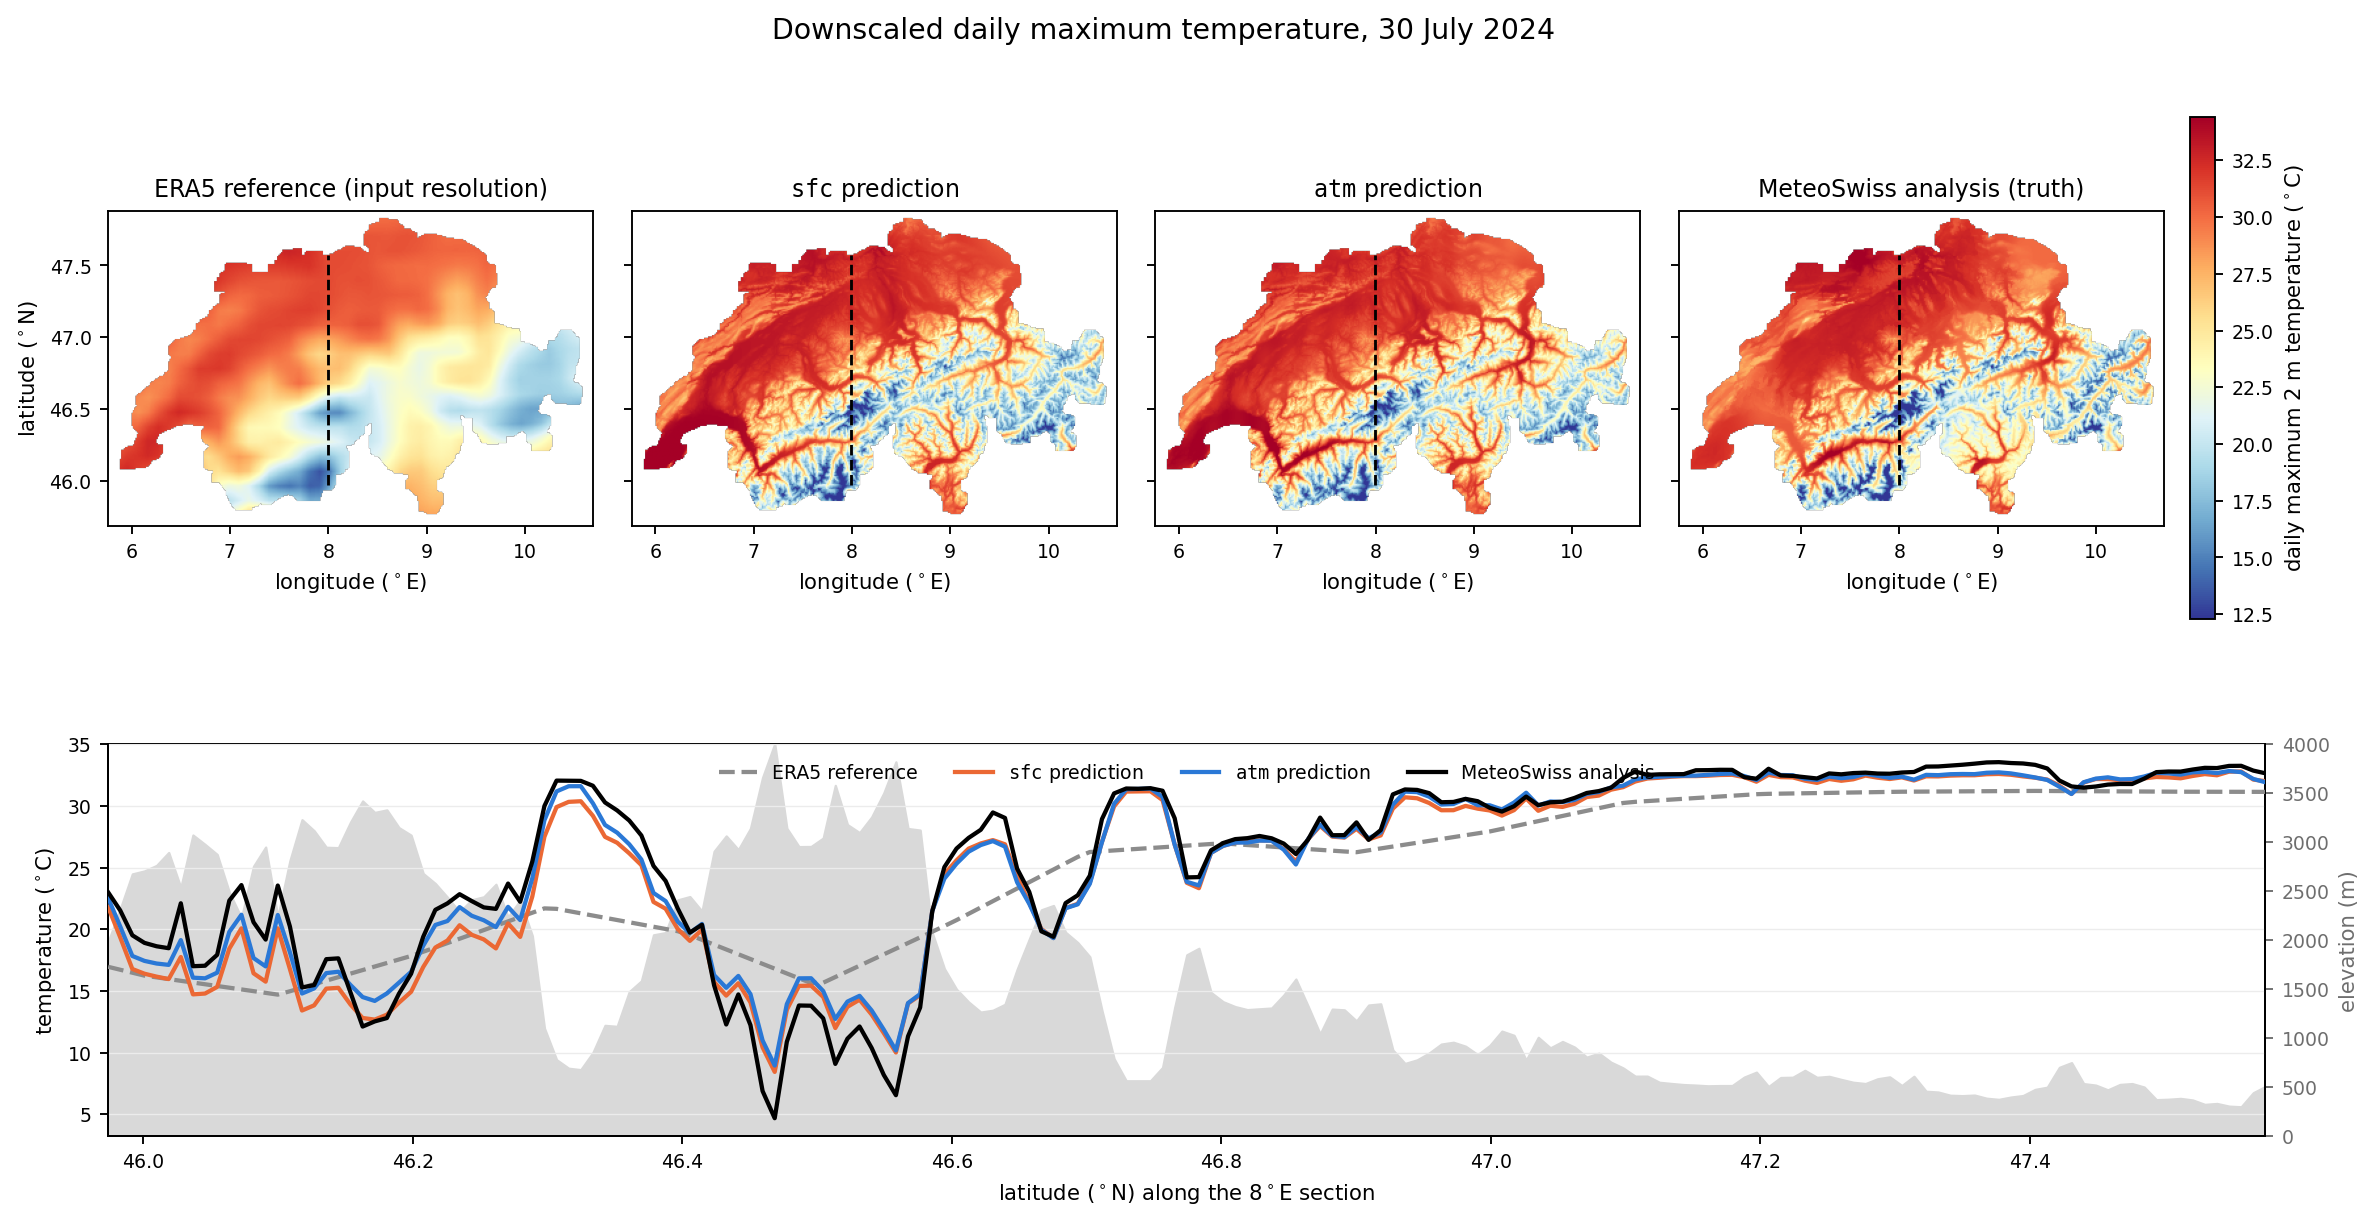
\includegraphics[width=0.74\textwidth]{images/tmax_spatial_section_warm.png}}

\caption[Downscaled field and temperature profile along a terrain section]{Downscaled field and temperature profile along a terrain section. On the top left of both figures we have the coarse-grid ERA5-Land surface temperature reference. On the top right the ground-truth MeteoSwiss Tmax field. In between the predictions for the surface and the atmospheric models. Below we have a south-to-north cross-section over the terrain and its temperature profile. These snapshots of two difficult days of the year show how well the temperature models are able to reconstruct the fine resolution of the terrain and the temperature field. The atmospheric model is able to follow the terrain profile more closely than the surface model. On the cold-weather day the surface model shows significant deterioration over the flat terrain of the Plateau while the atmospheric model is able to follow the ground truth. On the warm day both models are able to follow the terrain profile and the ground truth.}

\label{fig:single-tmax-spatial}

\end{figure}



Upon studying these two figures we notice a distinct difference in the reference forecast. Over the relief the reference is off by many degrees on both days, but that error is systematic, tied to the smoothed orography, and both models correct it in winter and summer alike. The offset we observe in winter over the Plateau is a different failure: there the target temperature runs about three degrees warmer than anything the reference field suggests. This offset, occurring only on the cold day and on the plateau originates in the daily conditions rather than in the missing orography. \texttt{sfc}, whose only meteorological signal is the surface temperature field cannot detect the systematic error and inherits the bias from the reference; \texttt{atm} can pick it up from the atmospheric context and follows the trends of the target.  On the warm day no such departure occurs and the two models are nearly equivalent. The surface input therefore suffices while the fine-scale truth follows the coarse field in a predictable way, and fails where the two decouple. Two chosen days are only illustrations, but \fref{fig:single-tmax-decoupling} extends these observations to the whole domain. It splits the observations into two elevation bands, below $600\,\mathrm{m}$ and above $2000\,\mathrm{m}$, and plots the monthly MAE for the reference and the two $30$-epoch models. The seasonality of the error is clear: the reference error is largest in the cold months. The atmospheric model only shows a slight increase of error for the cold months, while the surface model approaches the reference error in the cold months. This observation is equally valid for the lowlands and the high Alps therefore the origin is seasonal rather than geographic. The effect is even more pronounced when observing the holdout data 2024 (thin lines), where in the cold months the surface model and the reference are nearly identical.

\FloatBarrier

\begin{figure}[H]

\centering

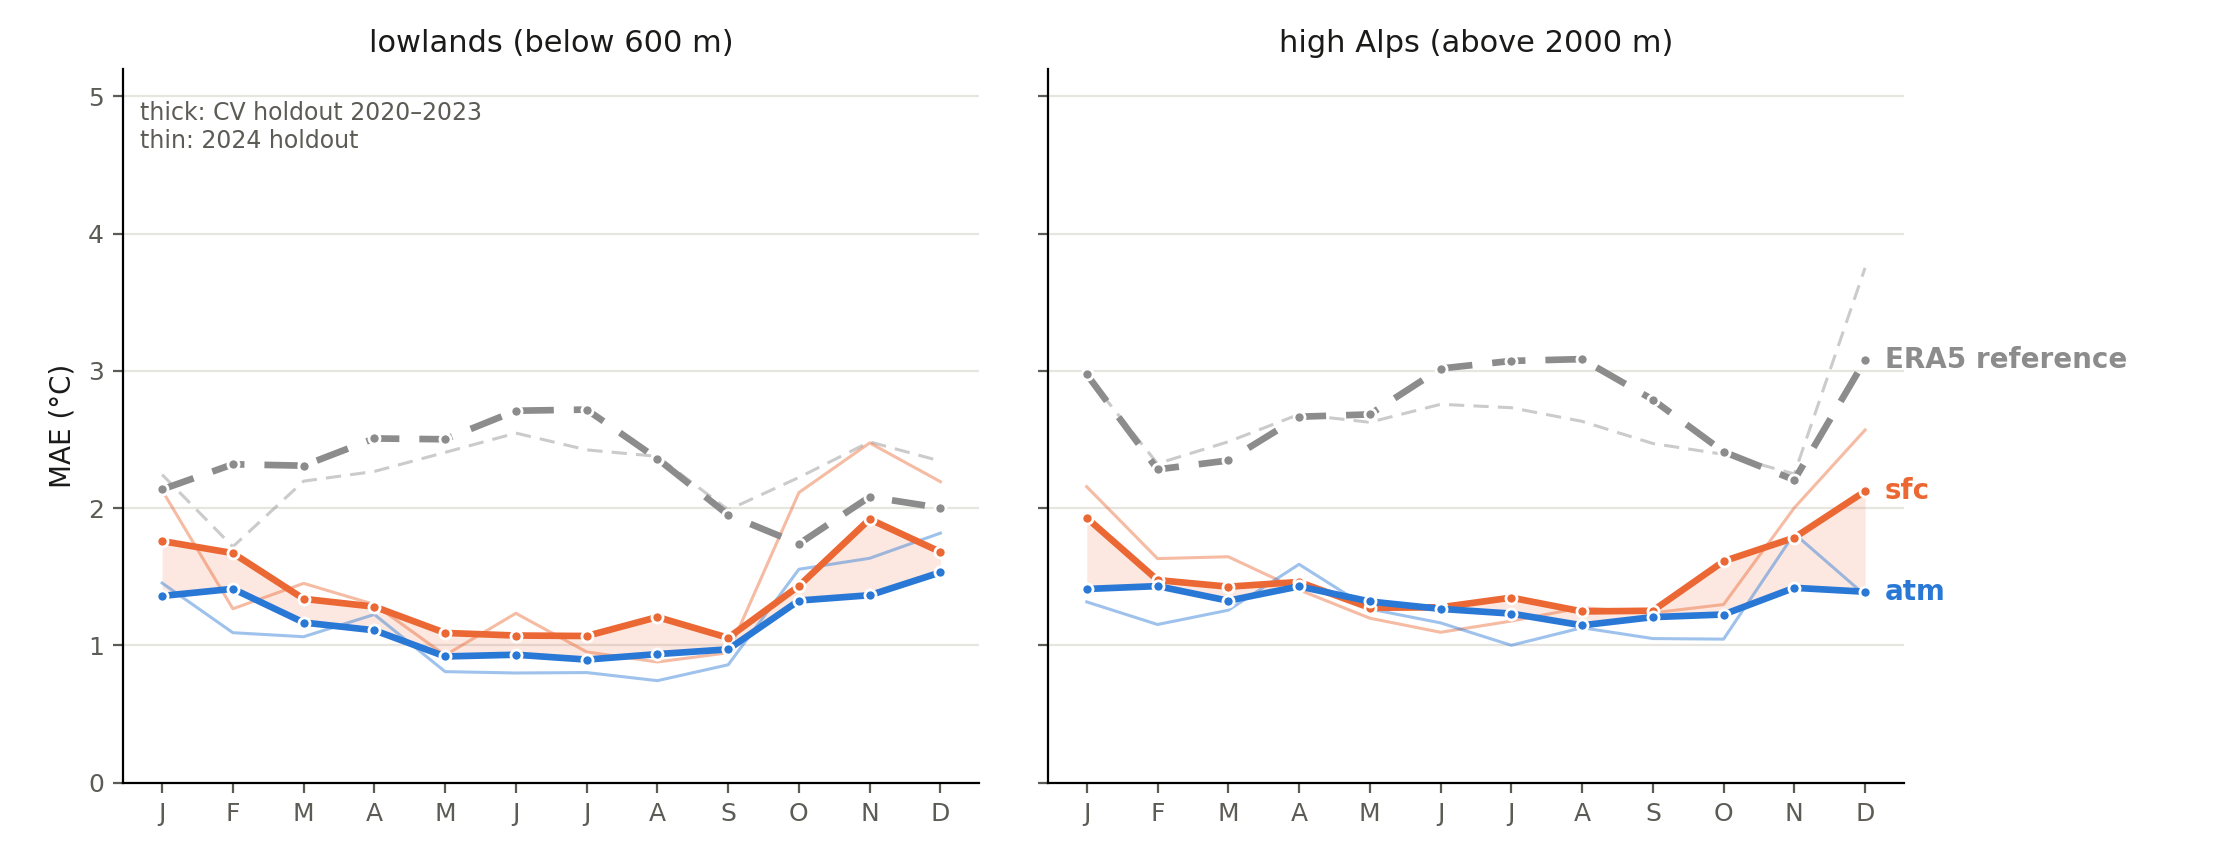
\includegraphics[width=0.9\textwidth]{images/tmax_seasonal_decoupling.png}

\caption[Seasonal decoupling of the surface input]{Seasonal decoupling of the surface input, read from the monthly MAE for the reference and the two $30$-epoch models \texttt{sfc} and \texttt{atm} over the lowlands (left, below $600\,\mathrm{m}$) and the high (right, above $2000\,\mathrm{m}$). Thick lines: the CV holdout 2020--2023, so each month is backed by four years; thin lines: the 2024 holdout. Both models stay well below the reference in every month of both bands. The systematic relief error is corrected year-round,  while the gap between \texttt{sfc} and \texttt{atm} (shaded) opens in the cold months and closes in summer, in both bands}

\label{fig:single-tmax-decoupling}

\end{figure}



\subsection{Model Selection}\label{subsec:single-tmax-geography}

\fref{fig:single-tmax-maecrpsmaps} maps both error metrics MAE and CRPS for the sfc and atm models and for the two atmospheric models with extended training. The same terrain signature appears in every panel: the overall error concentrates along the inner-Alpine valley floors and is lowest over the Plateau. The performance improvement from left to right is visible over the whole domain rather than confined to any one region. Longer training leads to significant improvements and starts, for the wind model, to reduce the error even in the valleys (green circles). CRPS and MAE agree on this spatial pattern. \fref{fig:single-tmax-windgain}, the direct comparison between the two extended-budget atmospheric models, highlights this positive impact of the wind input. So the improvement is strongest where the downscaling is hardest, along the inner-Alpine valley systems, and weakest along the Jura crest. The wind input is therefore not a general improvement, but a targeted one that helps most where it is needed. On average the wind channels buy little, a median gain of $+0.03\,^{\circ}\mathrm{C}$ per grid point with an improvement at $70\,\%$ of them, and the gain concentrates along the Rh\^one, Ticino, Grisons and Alpine Rhine valleys while the Jura crest is ceded. It is also a caution against reading permutation importance as the whole story: the $u$ and $v$ groups score near the bottom of the wind model's own importance ranking (\fref{fig:app-fi-sel-tmax}), yet carry a locally valuable signal that the global average hides.

\begin{figure}[H]

\centering

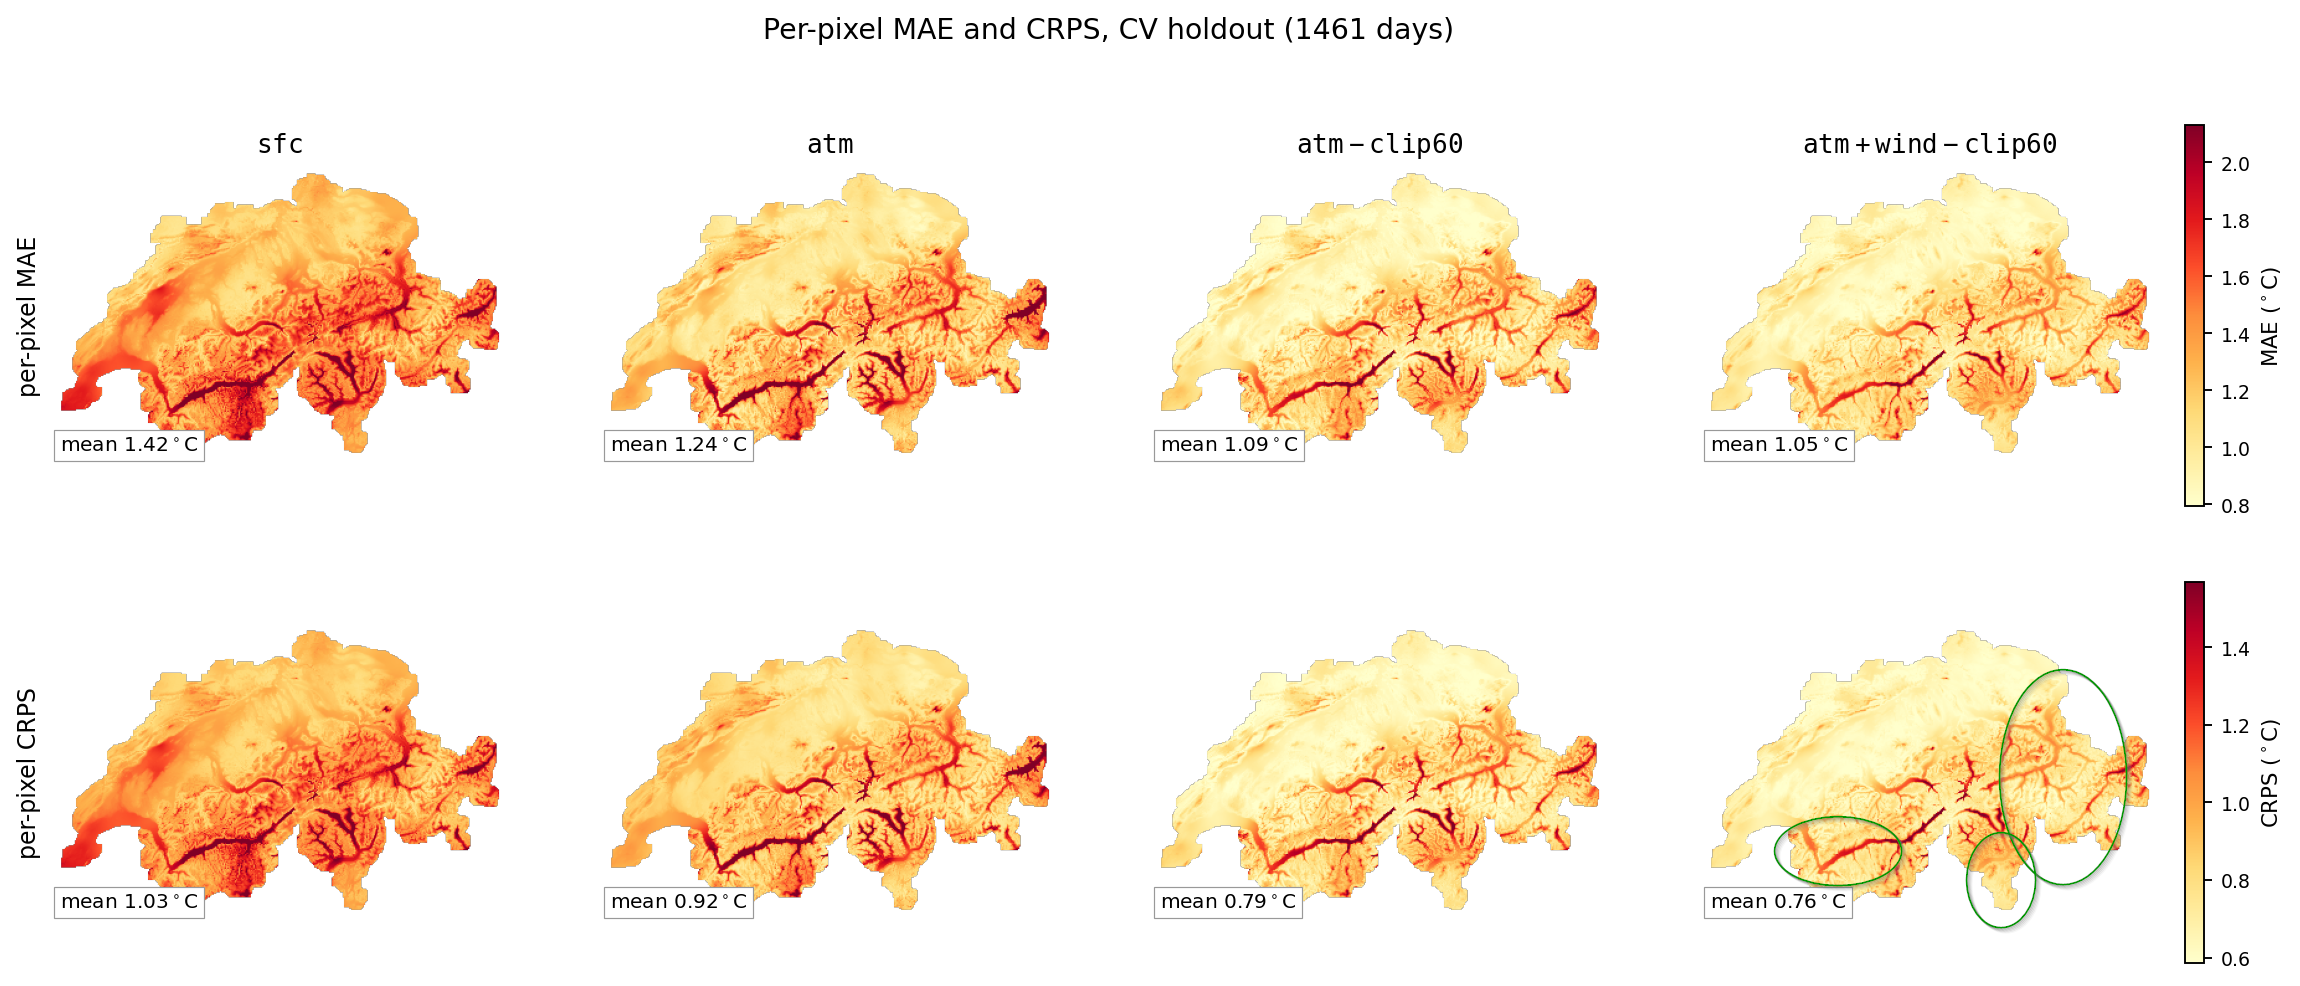
\includegraphics[width=\textwidth]{images/tmax_mae_crps_maps.png}

\caption[Per-pixel MAE and CRPS across four configurations]{Per-pixel MAE and CRPS over the CV holdout, for the two reference models (\texttt{sfc}, \texttt{atm}) and the two extended-budget atmospheric models (\texttt{atm-clip60}, \texttt{atm+wind-clip60}). Each row shares one colour scale, set to the 1st and 99th percentiles of the pooled distribution; the domain mean is given in each panel.}

\label{fig:single-tmax-maecrpsmaps}

\end{figure}







\begin{figure}[H]

\centering

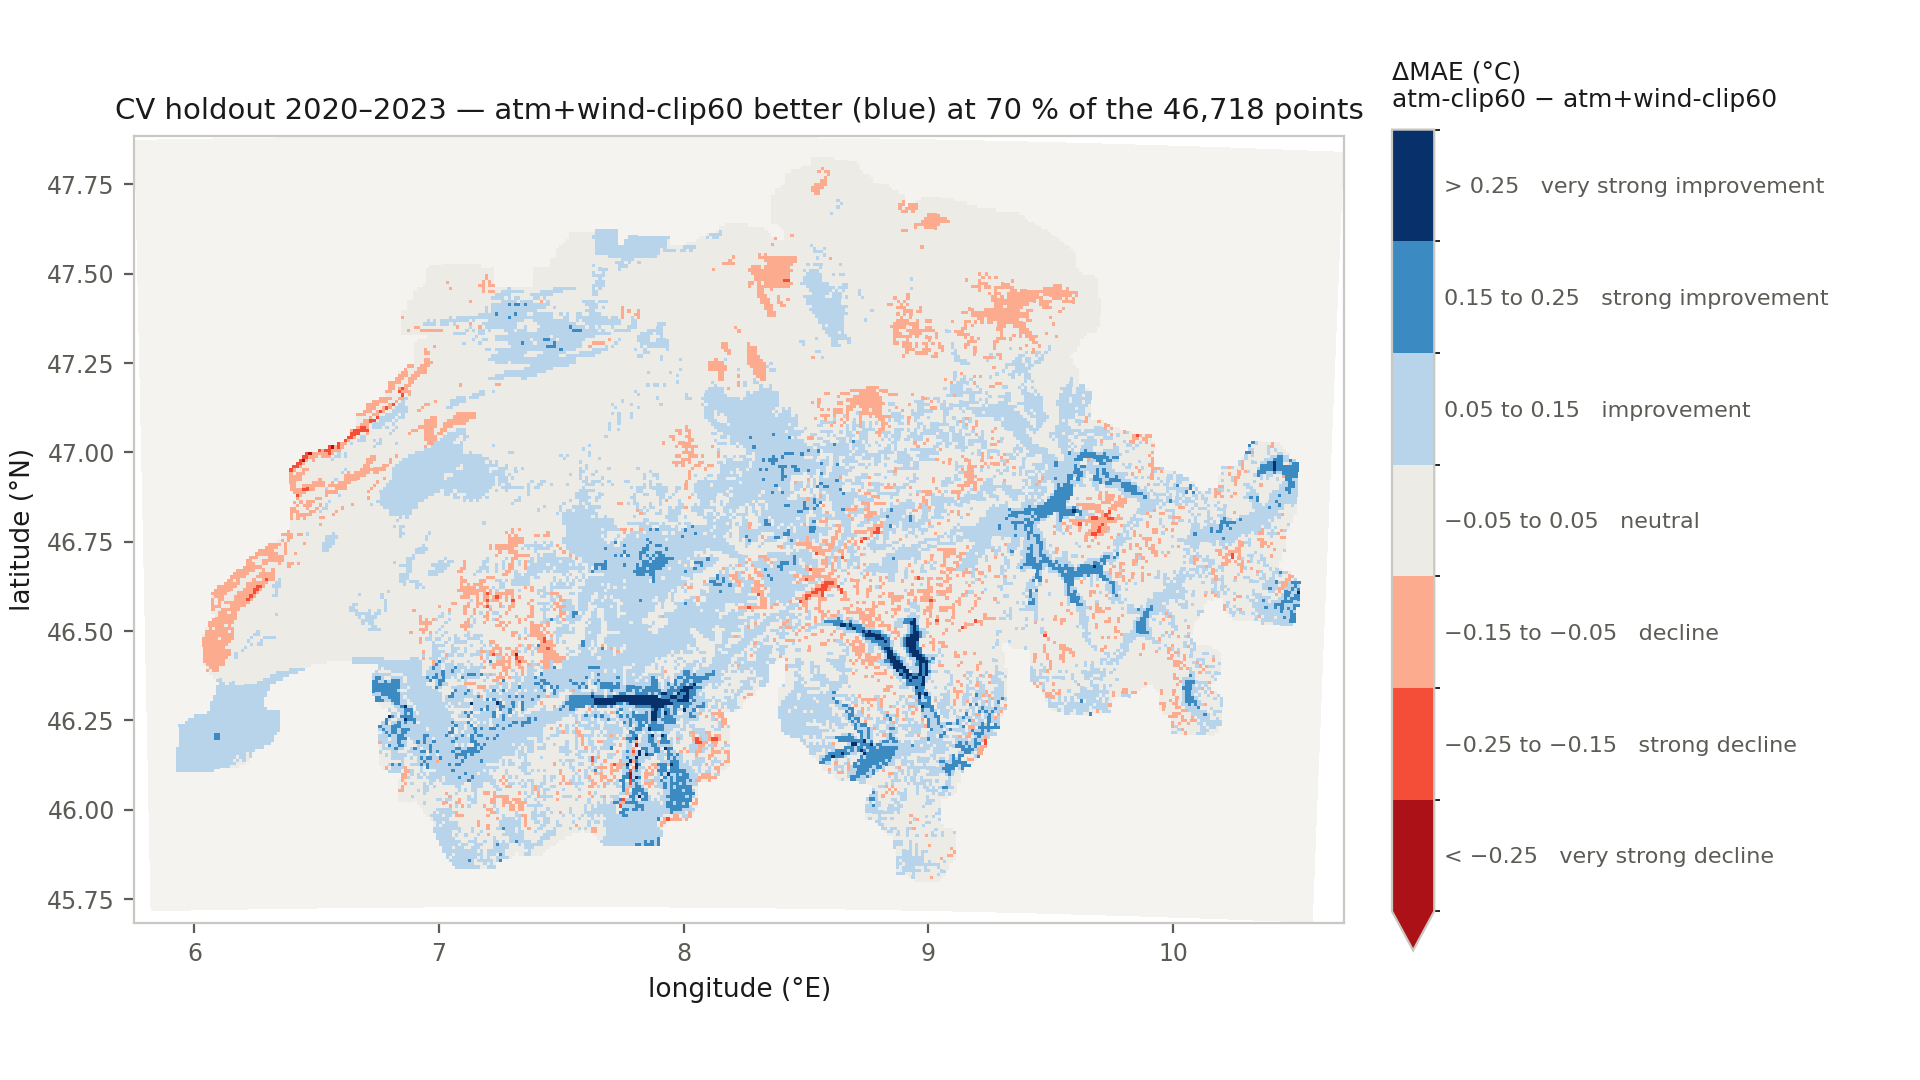
\includegraphics[width=0.9\textwidth]{images/tmax_wind_gain_map.png}

\caption[Where the wind input pays off]{Per-grid-point MAE saved by \texttt{atm+wind-clip60} over \texttt{atm-clip60} on the CV holdout. The gain concentrates along the inner-Alpine valley systems and 70\% of the points are improved. Loss is observed on isolated regions including some high altitude peaks and systematically and along the western border of switzerland.}

\label{fig:single-tmax-windgain}

\end{figure}






On this evidence we choose from here on to focus on the \texttt{atm+wind-clip60} model as the best performing model, and report the remaining results on it. The error of the selected model against terrain height and terrain position is shown in \fref{fig:single-tmax-terrain}. 



Every comparison in this subsection, and the choice itself, rests on the CV holdout, so the final selection between \texttt{atm-clip60} and \texttt{atm+wind-clip60} consumes only the training span; the unseen year entered the argument beforehand only through the aggregate generalisation check of \sref{subsec:single-tmax-headline} and the feature-importance study of \sref{subsec:single-tmax-fi}, which both are scored on 2024. The subsections that follow reverse the roles and report the selected model on 2024, as an example for the regime in which it would actually be deployed. This introduces new weather conditions the model has never seen, so the evaluation is a genuine test of how that specific choice generalises.



\subsection{Model Evaluation and Generalisation}\label{subsec:single-tmax-unseen}



\begin{figure}[H]

\centering

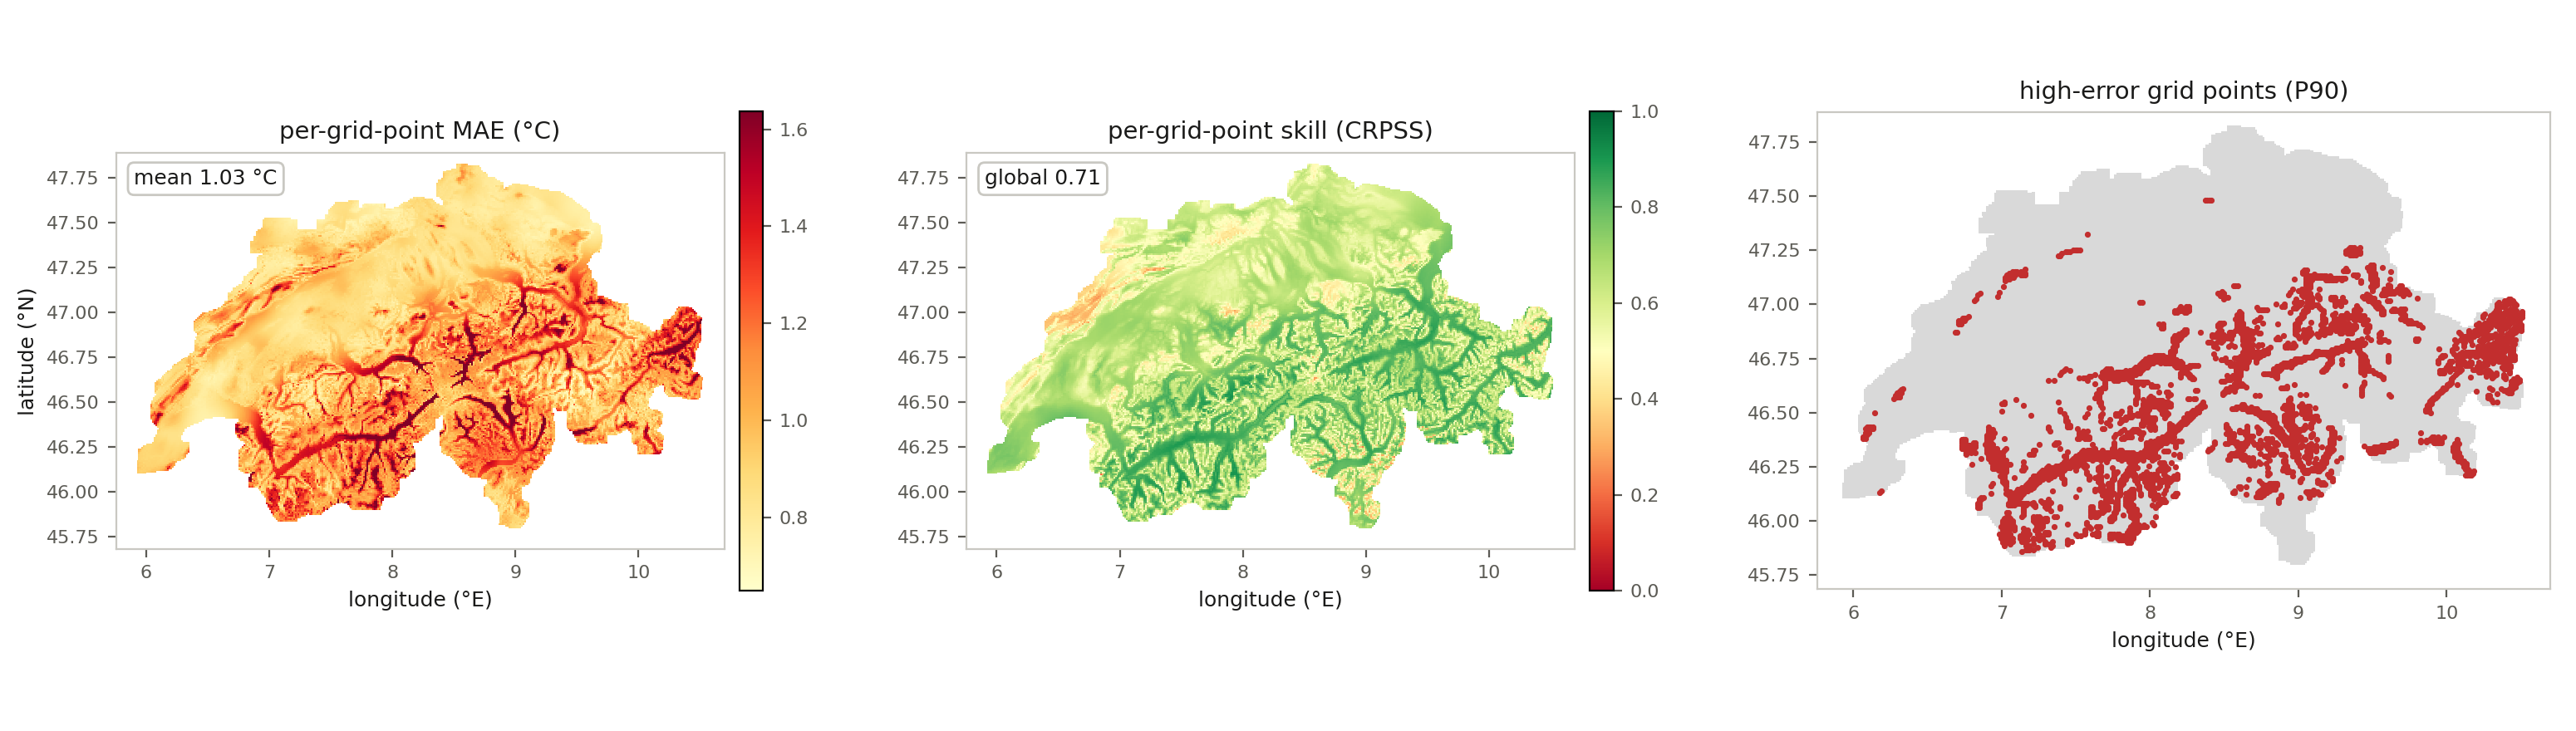
\includegraphics[width=\textwidth]{images/tmax_wind_2024_maps.png}

\caption[Where the error lives on the map]{Where the error lives on the map: \texttt{atm+wind-clip60} evaluated on the 2024 holdout. Per-grid-point MAE (left), per-grid-point skill against the bilinear ERA5-Land reference (centre), and the grid points above the 90th error percentile (right). The high-error set traces the inner-Alpine valley systems and some ridgelines, as well as the peak ridges in the Jura area. The Jura crest is the only region where the model only provides a marginal improvement over the reference.}

\label{fig:single-tmax-maemap}

\end{figure}



In the generalisation regime, the model reaches a global skill of $0.71$ against the bilinear ERA5-Land reference, with a MAE of $1.03\,^{\circ}\mathrm{C}$, slightly better than on the training span. The high MAE zones in \fref{fig:single-tmax-maemap} confirm the pattern of the CV maps: the lowlands sit at $0.7$--$0.9\,^{\circ}\mathrm{C}$ while  the inner-Alpine valley floors and ridgelines present the highest $10\,\%$ of errors. However when observing the  skill panel, it becomes clear that the model scores highest along the very valleys where its absolute error is largest. This is a direct result of the reference completely lacking accuracy in these regions. The lowest skill of the model is observed in the northwest Jura area.



When looking at the domain mean bias we can observe that the model has a tendency to overestimate temperatures. This bias grows from $+0.08\,^{\circ}\mathrm{C}$ on the CV span to $+0.23\,^{\circ}\mathrm{C}$ on 2024. \fref{fig:single-tmax-biasdrift} visualises the drift by calendar month: the 2024 curve sits above the CV curve in every month of the year, by $0.15\,^{\circ}\mathrm{C}$ on average and without seasonal concentration. The drift therefore behaves as a near-constant offset through the year.



\begin{figure}[H]

\centering

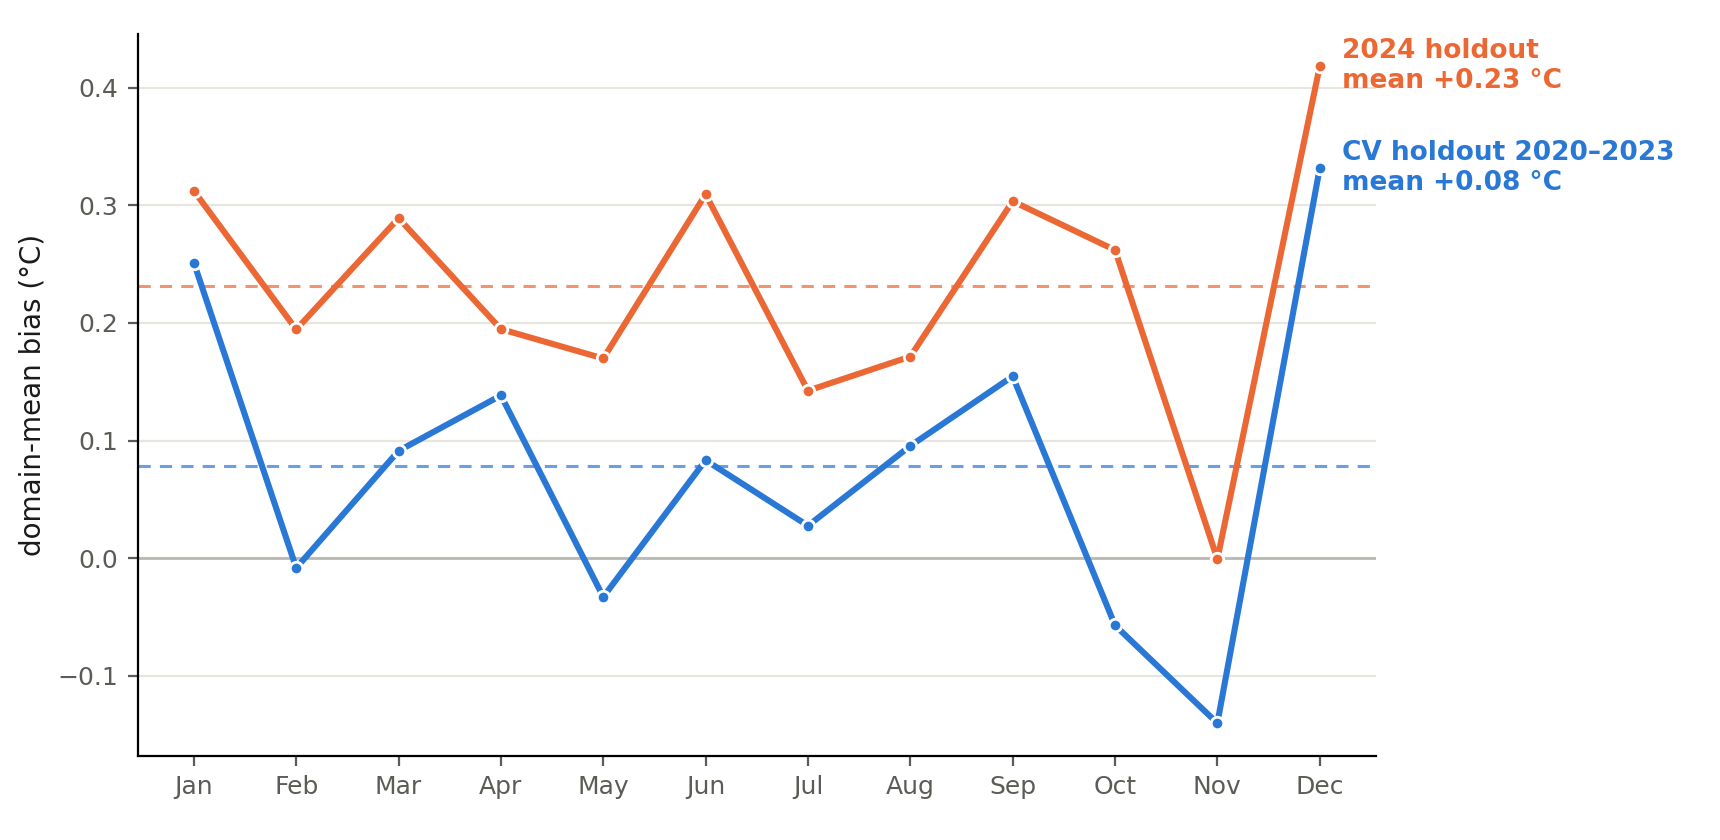
\includegraphics[width=0.9\textwidth]{images/tmax_bias_drift.png}

\caption[The warm drift on the unseen year]{The warm drift on the unseen year, read from the monthly domain-mean bias of \texttt{atm+wind-clip60} on the CV holdout and on 2024. Dashed lines mark the regime means. This shows that the warm drift on 2024 is nearly constant through the year.}

\label{fig:single-tmax-biasdrift}

\end{figure}



\subsection{Calibration and Distribution}\label{subsec:single-tmax-calibration}



\begin{figure}[H]

\centering

\subfloat[CV holdout 2020--2023, single-fold $\sigma$]{%

  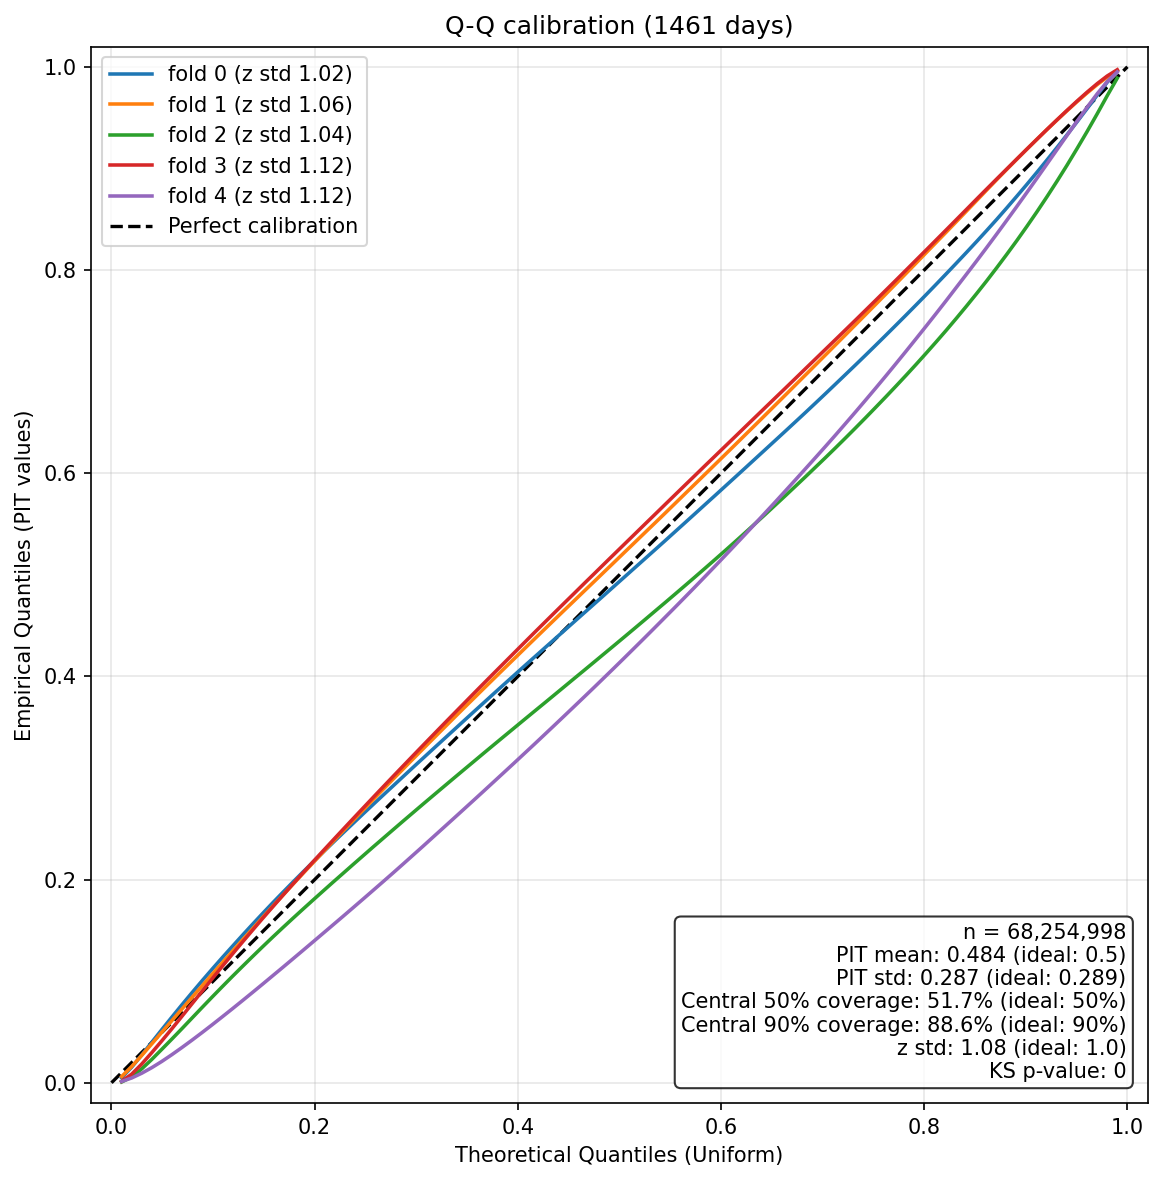
\includegraphics[width=0.46\textwidth]{images/results/tmax__qq_calibration__eval_cv__lbclip_wind.png}}\hfill%
\subfloat[2024 holdout, five-fold ensemble $\sigma$]{%

  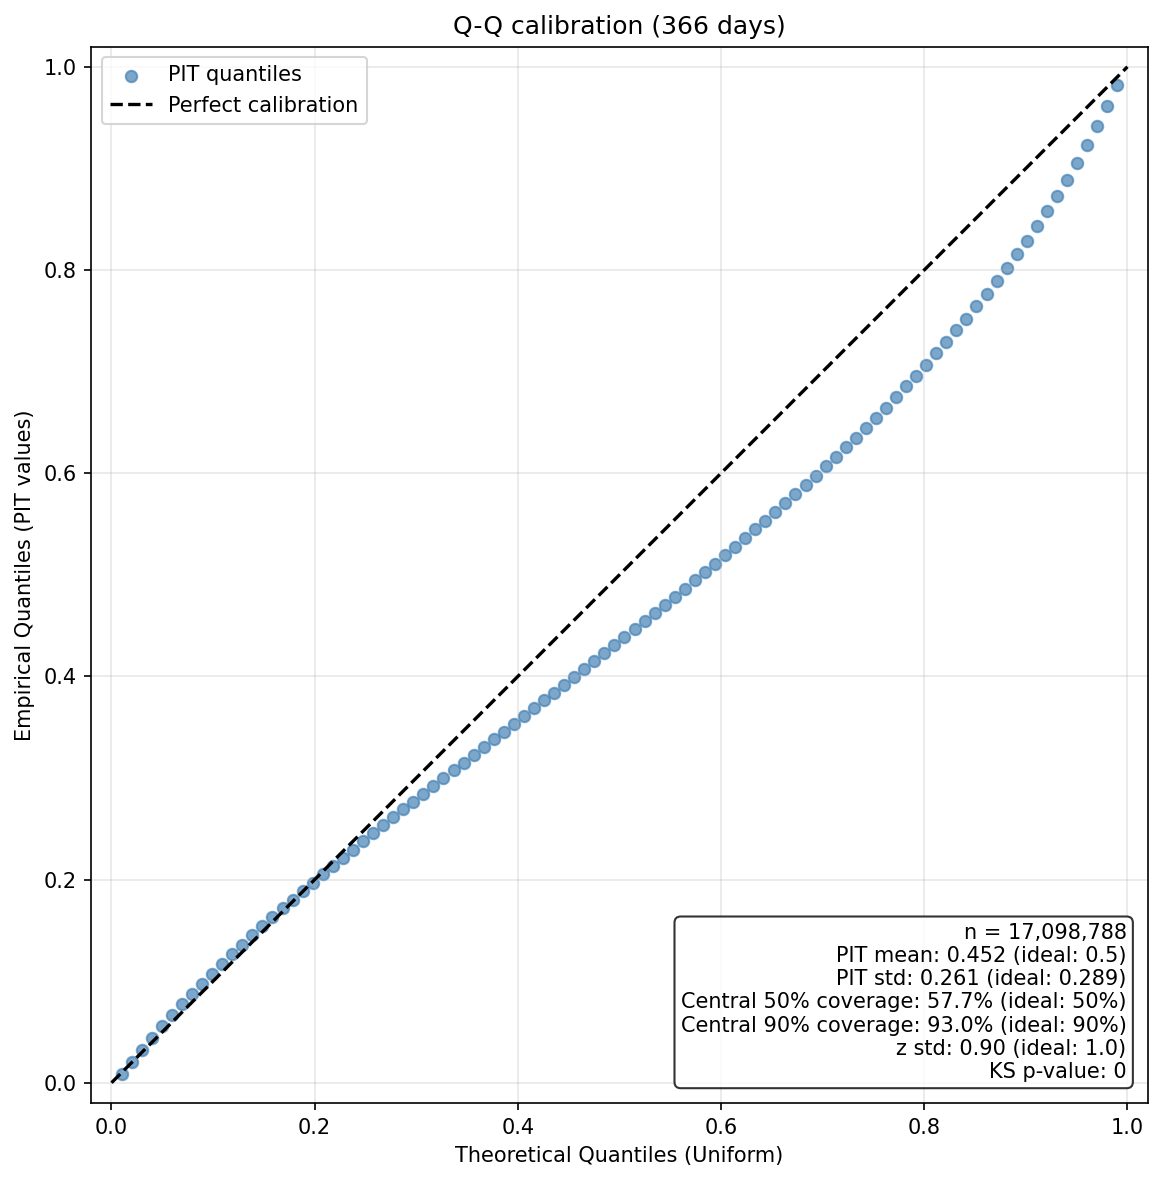
\includegraphics[width=0.46\textwidth]{images/results/tmax__qq_calibration__eval_2024__lbclip_wind.png}}

\caption[PIT calibration of the selected model across regimes]{PIT Q--Q calibration of \texttt{atm+wind-clip60} under both regimes. The CV panel draws one curve per fold, each fold scoring only the block it was held out from, so the spread between the curves is the disagreement between five separately trained models; the 2024 panel draws the single curve of the five-fold ensemble. }

\label{fig:single-tmax-pit}

\end{figure}



Over 2020--2023 the nominal $50\,\%$ and $90\,\%$ intervals capture $51.7\,\%$ and $88.6\,\%$ of the observations (\fref{fig:single-tmax-pit}). On 2024 they capture $57.7\,\%$ and $93.0\,\%$: the intervals are wider than the errors require, resulting in a conservative uncertainty estimate.



The PIT mean moves the same way, $0.48$ on the CV holdout against $0.45$ on 2024, which is the warm drift of \fref{fig:single-tmax-biasdrift} seen from the calibration side. The spread is still informative where it matters: it grows with the error it has to cover, at $r = 0.66$ on 2024 and $r = 0.55$ on the CV holdout. Across a range of more than $50\,^{\circ}\mathrm{C}$ the predicted density follows the observed one (\fref{fig:single-tmax-dist}); the exception is the warm tail, where every configuration puts too much probability above $30\,^{\circ}\mathrm{C}$.



\begin{figure}[H]

\centering

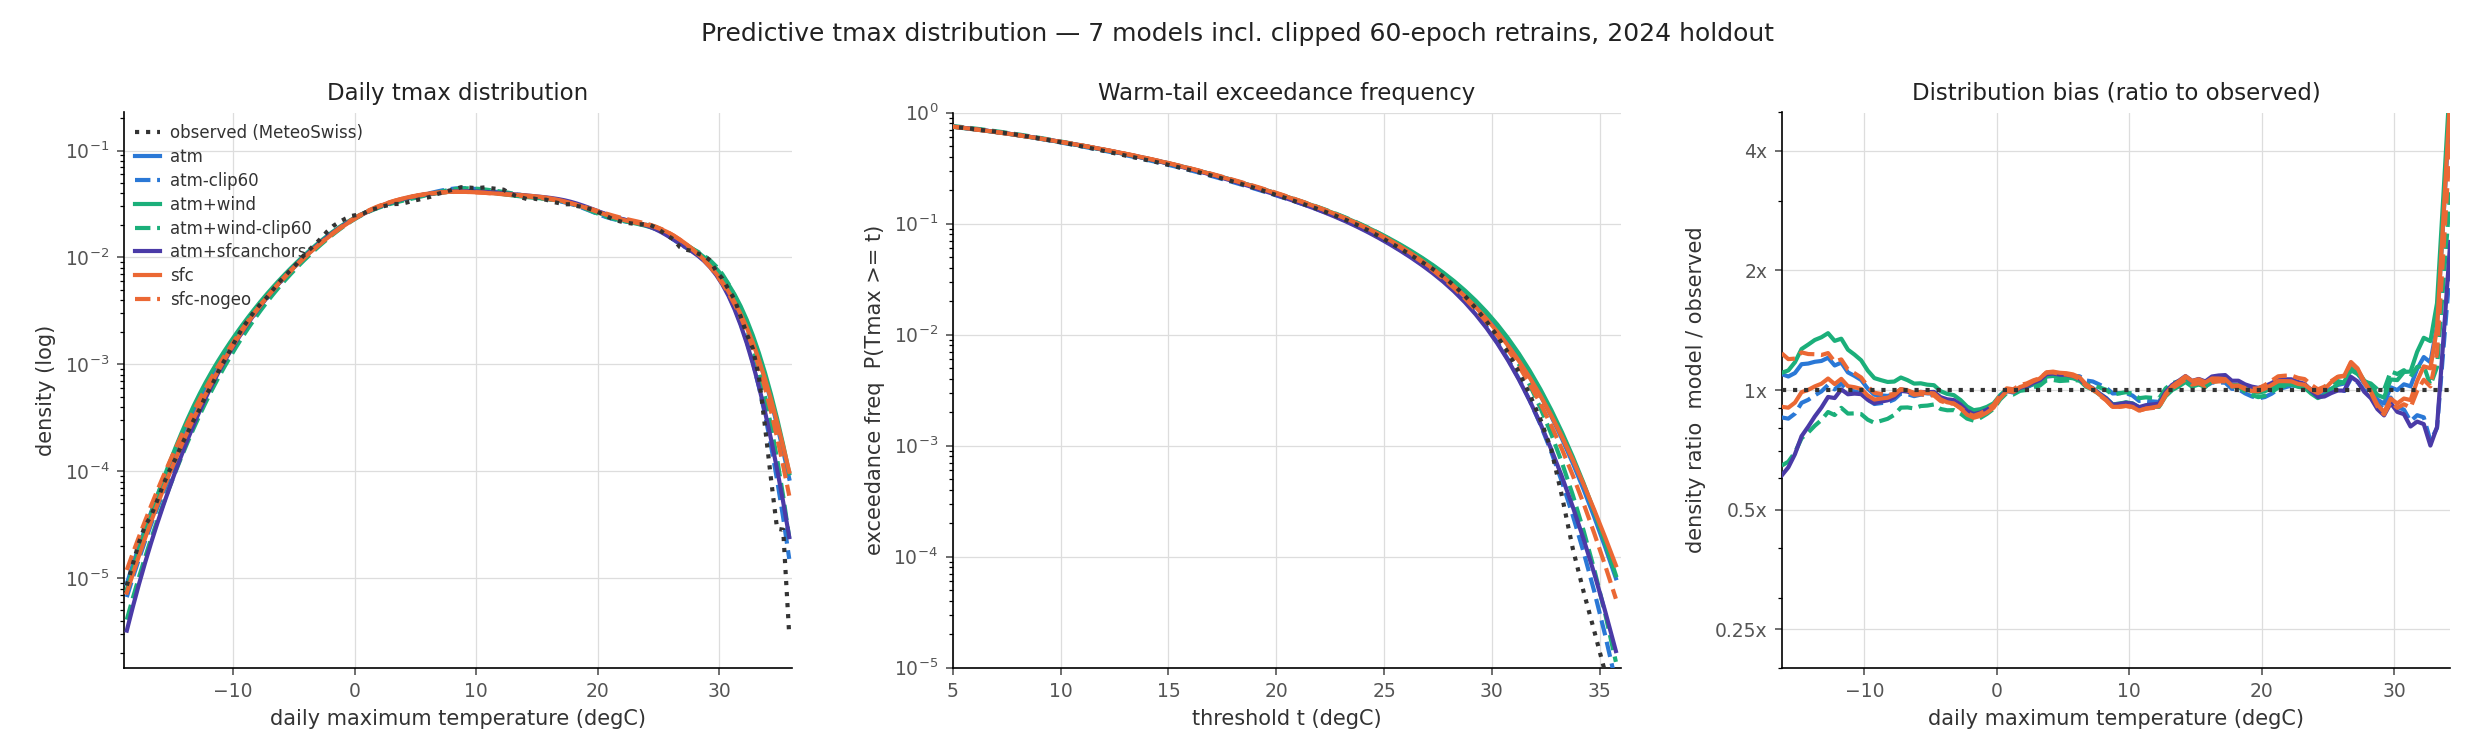
\includegraphics[width=\textwidth]{images/results/tmax__tmax_distribution_overlay_with_clip60_2024__tmax_model_comparison__ALL.png}

\caption[Predicted vs observed temperature distribution, 2024]{Predicted against observed daily-maximum temperature distribution over all points and days of 2024, for all seven models: log-density, warm-tail exceedance frequency, and the model-to-observed density ratio.}

\label{fig:single-tmax-dist}

\end{figure}

\subsection{Discussion}\label{subsec:single-tmax-discussion}



The atmospheric input generalises rather than merely fits the training years: all five atmospheric configurations hold or slightly improve their scores on 2024, a year no fold saw, relative to the CV holdout they were tuned against, while both surface configurations get worse (\fref{fig:single-tmax-slope}). An overfit model would degrade on unseen data, so this is the behaviour of a model that learnt something about the atmosphere rather than about the four particular years it was trained on. The advantage is not spread evenly: the surface input already tracks the fine-scale truth when that truth follows the coarse field, and it is mainly in the cold season, when the two decouple, that only the atmospheric input can keep up (\fref{fig:single-tmax-decoupling}). Against the predecessor project of \textcite{passos}, whose strongest configuration reaches a skill of $0.52$ with a surface input trained on ten years, the comparison is loose, since the evaluation years, the exact methodology and the training spans all differ. The more meaningful number is the internal comparison: on the CV holdout, moving from this work's own \texttt{sfc} baseline ($0.60$) to the selected atmospheric model ($0.70$) raises the skill by $0.10$.



Within the atmospheric input, the wind channels are a local rather than a global asset. Permutation importance ranks them near the bottom (\fref{fig:app-fi-sel-tmax}), yet under the extended training budget they buy the decisive margin of improvement exactly along the hardest-to-predict valley systems (\fref{fig:single-tmax-windgain}). 

Weather persists from one day to the next, so consecutive days do not carry independent information and a year of them is worth less than its calendar length suggests. Correcting for that persistence leaves 2024 with roughly $220$ effectively independent days rather than $366$ (\eref{eq:neff}). On that reduced sample the selected model's warm drift on 2024 is $+0.23\,^{\circ}\mathrm{C}$ with a $95\,\%$ interval of $[+0.16, +0.30]$, so it is a systematic offset and not a peculiarity of the evaluated year. The same test on the CV span returns $+0.08\,^{\circ}\mathrm{C}$ with an interval of $[+0.04, +0.12]$: the model is warm in both regimes, and what 2024 adds is a threefold amplification rather than the offset itself. Its amplitude is smaller than the model MAE so it is not a major flaw, but it is present.

The model selection itself is close rather than clear-cut: \texttt{atm+wind-clip60} is the most accurate model on every metric in both regimes, and it is the model we select, but \texttt{atm-clip60} would be the more robust choice for a use case that values stability over the last few hundredths of a degree. It transfers to 2024 almost without bias ($-0.02$ against $+0.23\,^{\circ}\mathrm{C}$), its calibration barely changes between the regimes, its five folds agree more closely (\fref{fig:app-sigma-decomposition}), and it does so with $95$ instead of $155$ channels.

Two weaknesses survive all of the seven configurations: the inner-Alpine valley floors and the over-predicted warm tail above $30\,^{\circ}\mathrm{C}$. Neither is fixed by picking a different model from this comparison; both need a lever this work did not pull. On training, that lever is already visible in the results here: doubling the epoch budget alone was worth more than any input modification achieved, and every model in this comparison still trained on only four years of data. Scaling both further, a longer schedule and more years, is the most direct, untested route to closing the valley-floor gap. The warm tail is a different kind of failure and will not close the same way; it needs a dedicated fix, such as post-processing the upper tail, rather than more training.

 One limit applies to everything in this chapter. The Gaussian head predicts each target point on its own (\sref{subsec:meth-gaussian}). Every map is therefore a field of per-point means, and every $\sigma$ is the spread at that point alone. Reading the maps and checking the calibration point by point is sound. What cannot be checked here is whether the errors have the right spatial structure, because the model never predicts how the error at one point relates to its neighbour. The between-fold spread of \fref{fig:app-sigma-decomposition} does not fill that gap: it measures how far the five folds disagree at each point, not how neighbouring points move together. In this work we have not studied this effect. Autoregressive sampling would settle it: coherent draws from the trained model, compared against the observed fine-scale variance~\cite{bruinsma2023arcnp}.

One design choice looks wrong in hindsight, and it concerns the domain rather than the model. The context grid extends well beyond the national border, but the loss is formed only at target points inside Switzerland (\sref{objective}): of the $88\,800$ points of the temperature lattice, only $46\,718$ ever carry a gradient. The model is therefore supervised only inside the Swiss border. The border region is therefore fitted with support that stops abruptly. Nothing constrains what the field does just outside, so the last kilometres inside the border are interpolated partly from grid cells whose behaviour was never scored. Extending the supervised area some way beyond the border or even the whole target set would have removed that asymmetry, and the data for it is available. Seen from the cost side the same choice is also wasteful, since roughly $47\,\%$ of the effort spent in the RBF layer and the elevation MLP goes to points that never enter the loss (\sref{subsec:meth-cost}).

\subsection{Conclusion}\label{subsec:single-tmax-conclusion}



This chapter answers the two questions it set out to ask (\sref{sec:intro-questions}) for temperature. Meteorologically relevant features do improve accuracy and calibration over surface data: atmospheric input beats surface input on every metric, keeps improving rather than degrading on the unseen 2024 year, and the selected model, \texttt{atm+wind-clip60}, reaches a skill of $0.71$ and a MAE of $1.03\,^{\circ}\mathrm{C}$ with a small, well-behaved warm bias as its only significant caveat.


The model also learns physically meaningful structure rather than acting as a trained interpolator: it relies on lower-tropospheric temperature at the hours a warm front or a clear midday sky would matter, not on scaffold or coordinate channels, and this reliance is what lets it, unlike the surface models, generalise better to weather it never trained on. The remaining weaknesses are the MAE over the inner-Alpine valley floors, the warm tail, and the cold-season decoupling of surface-driven inputs.



\section{Precipitation Model}\label{sec:single-precipitation}




\subsection{Model Variants}\label{subsec:single-precip-variants}

In the presented models, two axes are studied: the training objective and the input feature set. Three runs share the
atmospheric input of the temperature study and differ only in the objective they minimise:
\texttt{precip-NLL}, \texttt{precip-CRPS} and \texttt{precip-FT-CRPS}. \texttt{precip-WIND} adds the
wind components to that same atmospheric input.

\texttt{precip-SFC-TP} replaces the atmospheric inputs with a pure surface
input including ERA5-Land total precipitation and daily-maximum $2\,\mathrm{m}$ temperature. \tref{tab:single-precip-variants} lists all five with the model names used throughout.

In this section the reference baseline is the bilinearly interpolated ERA5-Land total precipitation. To match the evaluation window of the observed target, the reference is rebuilt on a $06\,\mathrm{UTC}$ to $06\,\mathrm{UTC}$ window (\sref{sec:data-preprocessing}). The input channel of \texttt{precip-SFC-TP} keeps the $00\,\mathrm{UTC}$ window all atmospheric models were trained on.


\begin{table}[H]
\centering
\caption[The five precipitation runs]{The five precipitation runs. All share the architecture of
\sref{sec:meth-architecture}, the Bernoulli--Gamma head of \sref{subsec:meth-likelihoods} and the
setup of \tref{tab:meth-training-setup}; \texttt{precip-FT-CRPS} is a warm start run from the trained
\texttt{precip-NLL} model with the objective function based on CRPS.}
\label{tab:single-precip-variants}
\footnotesize
\begin{tabular}{|>{\raggedright\arraybackslash}p{2.8cm}|>{\raggedright\arraybackslash}p{5.2cm}|>{\raggedright\arraybackslash}p{3.2cm}|>{\raggedright\arraybackslash}p{1.0cm}|}
\hline
\textbf{Model name} & \textbf{Context input} & \textbf{Objective} & \textbf{Chan.} \\
\hline
\texttt{precip-NLL} & ERA5 pressure-level $z$, $t$, $q$ on six levels at five hours, plus scaffold &
mixture NLL, \mbox{\eref{eq:bg-ll}} & 95 \\
\hline
\texttt{precip-CRPS} & as \texttt{precip-NLL} & sampled CRPS, \mbox{\eref{eq:crps}} & 95 \\
\hline
\texttt{precip-FT-CRPS} & as \texttt{precip-NLL} & NLL, then $10$ epochs of CRPS & 95 \\
\hline
\texttt{precip-WIND} & as \texttt{precip-NLL}, with the wind components $u$ and $v$ added & mixture NLL & 155 \\
\hline
\texttt{precip-SFC-TP} & ERA5-Land total precipitation and daily-maximum $2\,\mathrm{m}$ temperature, plus
scaffold & mixture NLL & 7 \\
\hline
\end{tabular}
\end{table}



\subsection{Headline Metrics}\label{subsec:single-precip-headline}

\fref{fig:single-precip-slope} and \fref{fig:single-precip-slope-skill} plot each run from its CV-holdout score to its 2024 score. The values themselves are in \tref{tab:single-precip-headline}.

Every quantity plotted for the runs is a closed-form functional of the fitted Bernoulli--Gamma
distribution, evaluated per point-day: the predictive mean $\rho\alpha/\beta$ for the errors and the
rank correlation, $P(Y \geq 1\,\mathrm{mm})$ for occurrence and
$E[Y \mid Y \geq 1\,\mathrm{mm}]$ for intensity; the two skill scores combine these with the same
ERA5-Land reference the grey line carries. Thresholds enter only as events: $1\,\mathrm{mm}$ for
occurrence and intensity, the four category edges for the RPSS and never as a wet/dry decision
on the prediction. All statistics pool days and points together. 
\begin{figure}[H]
\centering
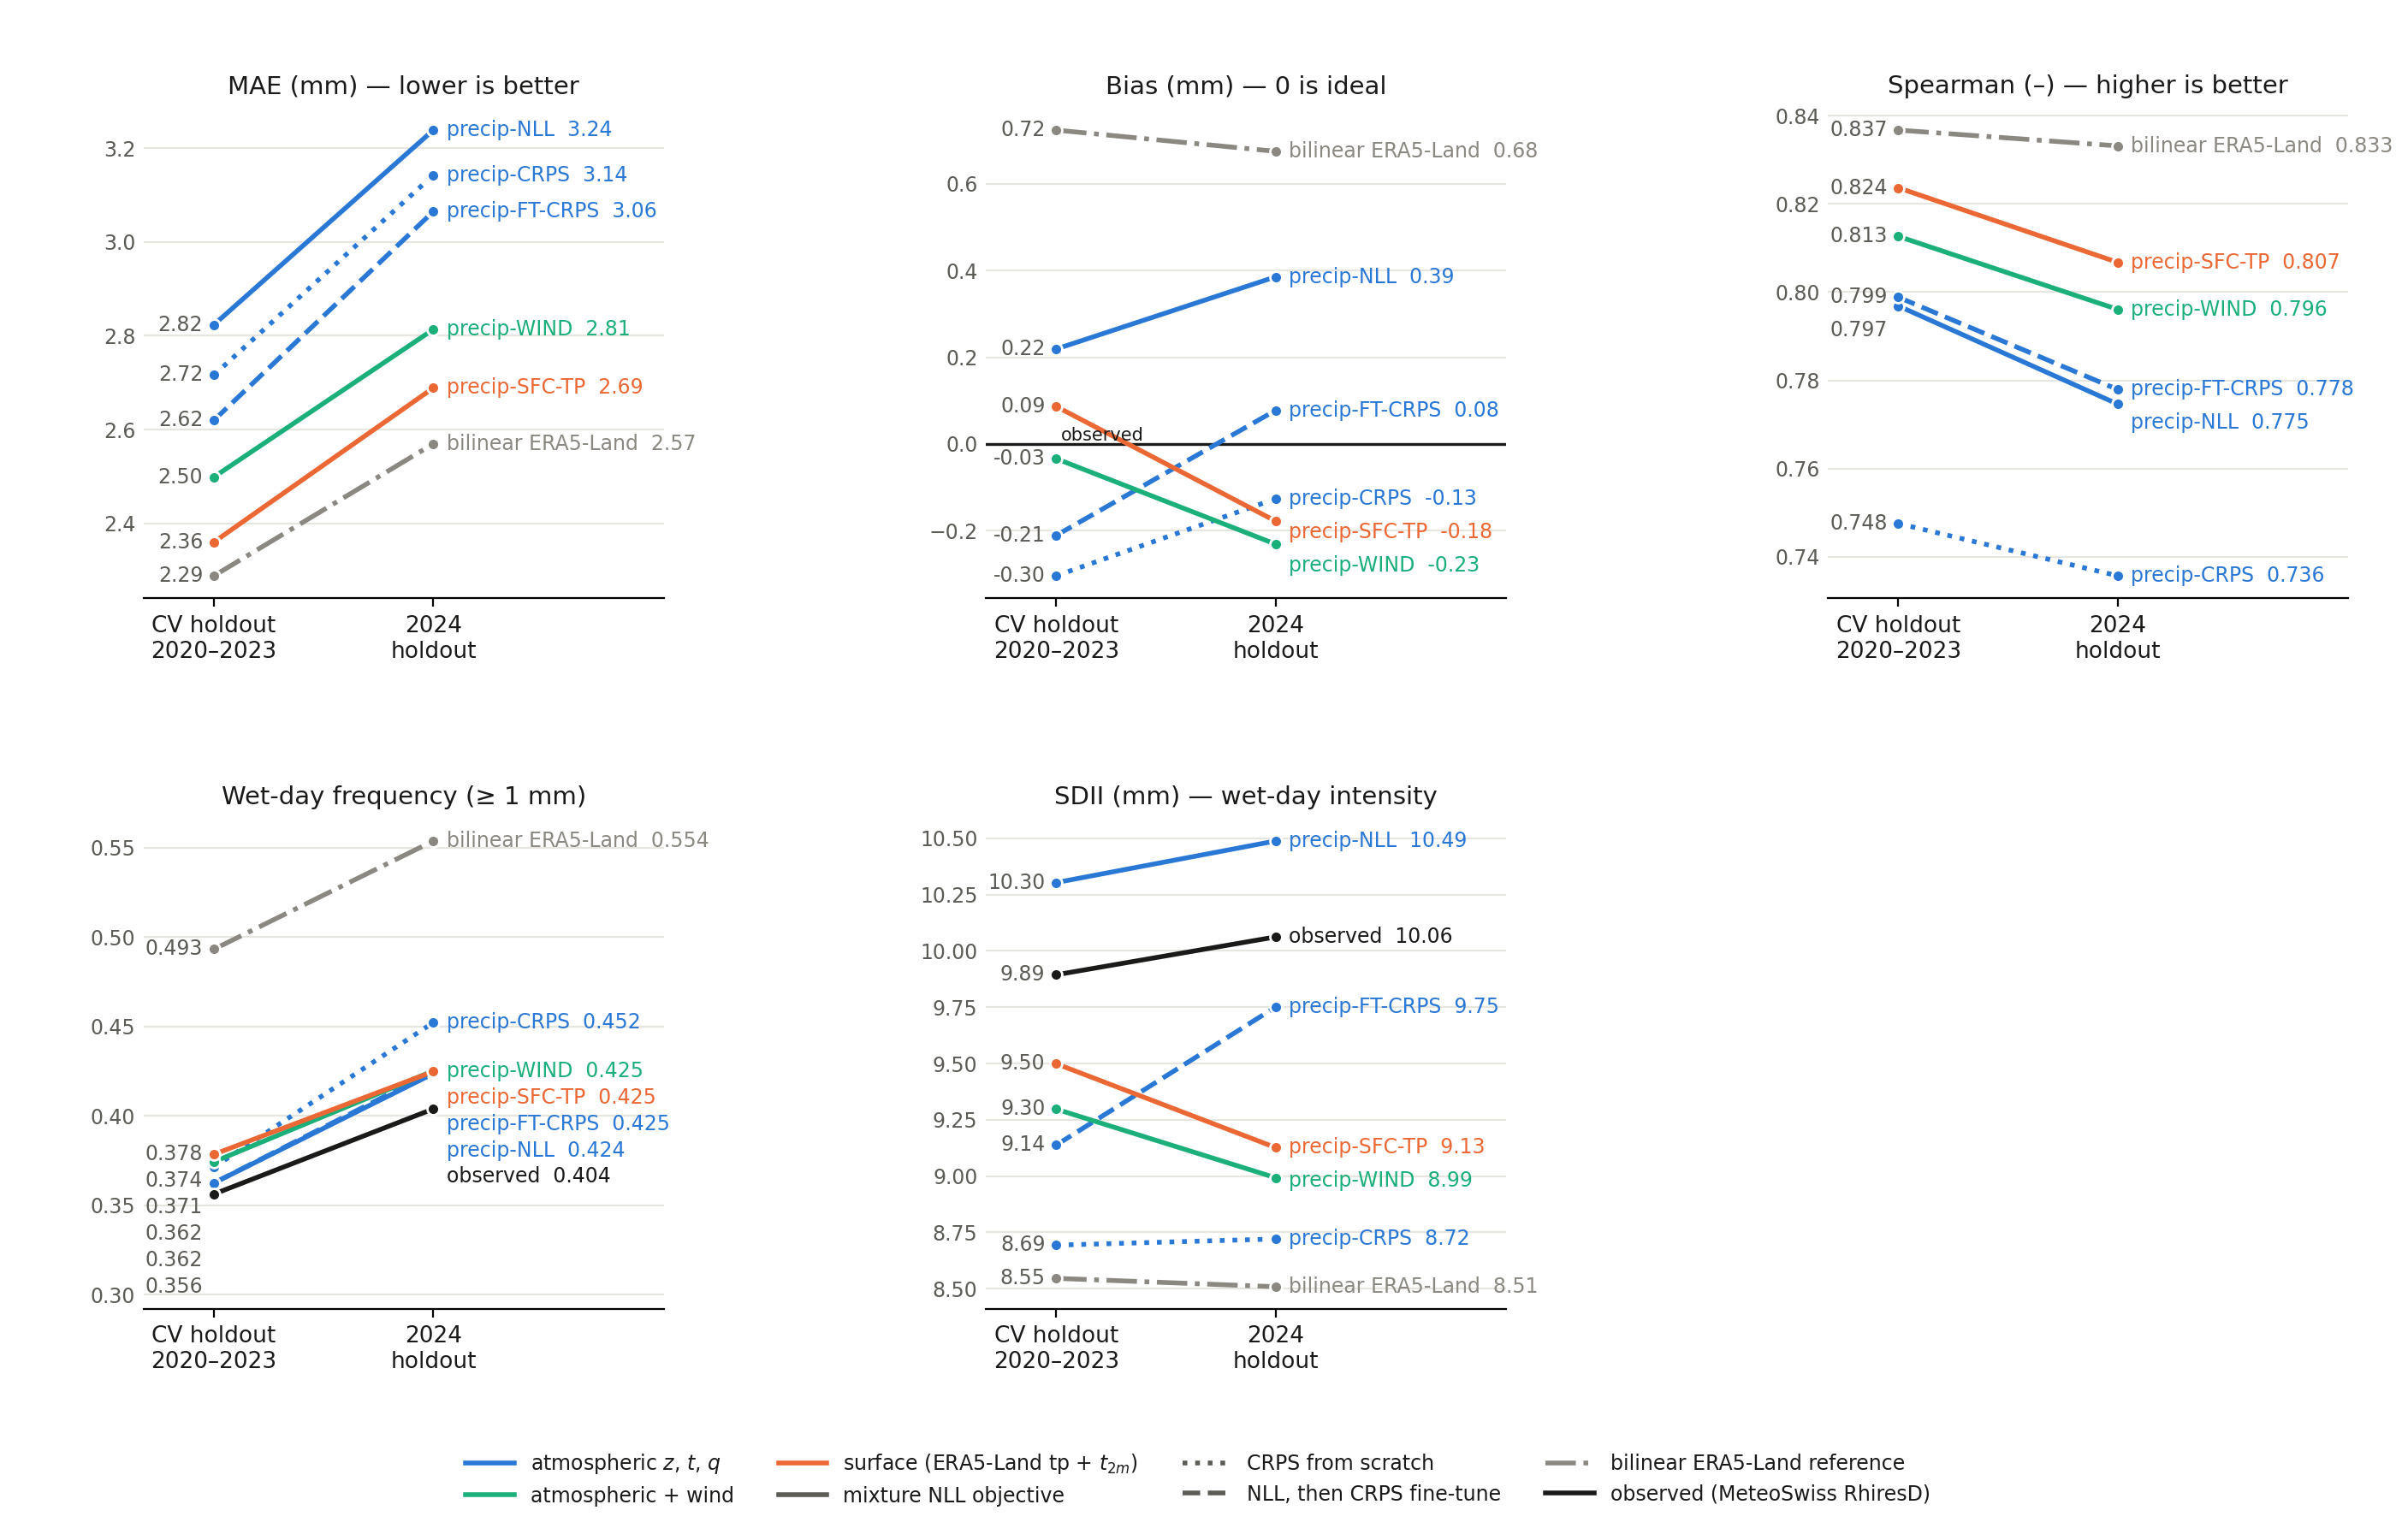
\includegraphics[width=\textwidth]{images/precip_regime_slope.png}
\caption[Accuracy of the precipitation runs, CV to 2024]{The scores of the five
precipitation runs from the CV holdout to the unseen year: the two error measures and the rank
correlation on the top row, occurrence and wet-day intensity below. Colour encodes the input family
and line style the training objective; the bilinear ERA5-Land reference is the grey line and the
observed target the black one.}
\label{fig:single-precip-slope}
\end{figure}

\begin{figure}[H]
\centering
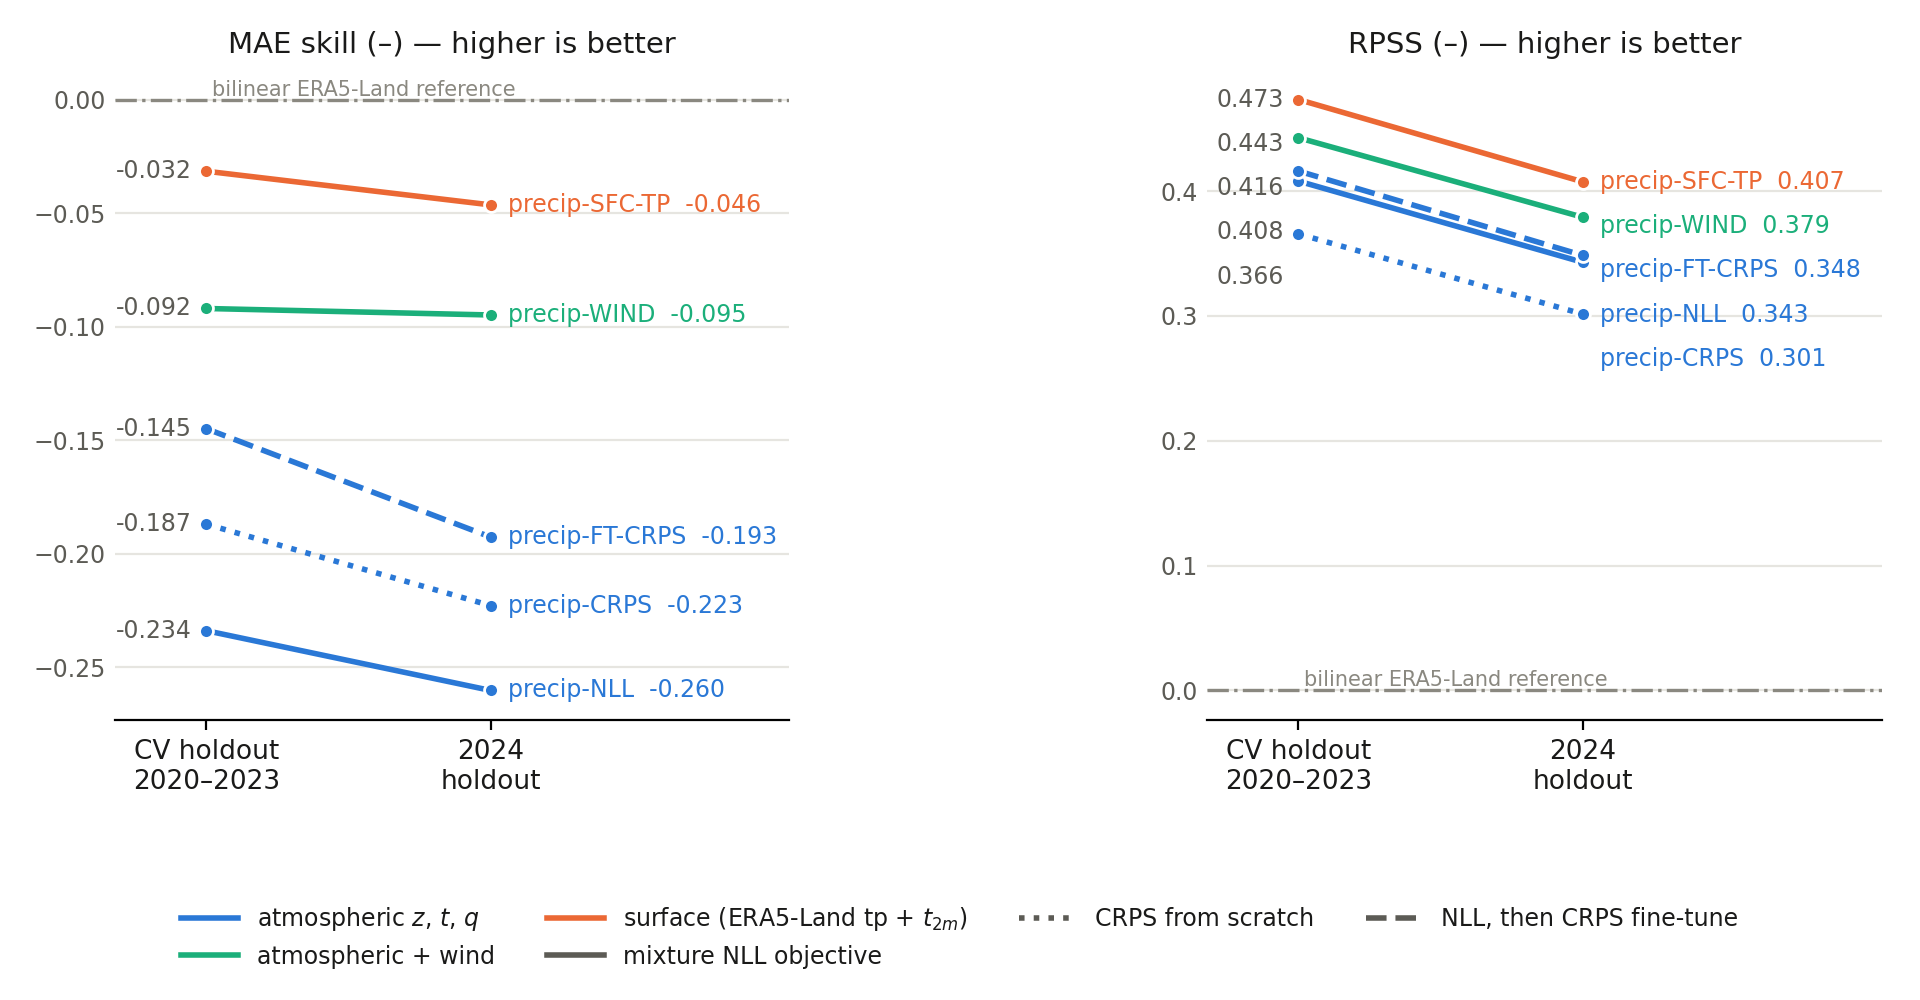
\includegraphics[width=0.8\textwidth]{images/precip_regime_slope_skill.png}
\caption[Skill of the precipitation runs, CV to 2024]{The two skill scores of the five runs over the
same two regimes, on the conventions of \fref{fig:single-precip-slope}. Both are defined against the
bilinear ERA5-Land reference, so the reference is the zero rule: the MAE skill of
\eref{eq:mae-skill} is negative for every run in both regimes, while the RPSS of \eref{eq:rpss} is
strongly positive for all of them. The two agree on the ranking apart from the two weakest runs, which swap places.}
\label{fig:single-precip-slope-skill}
\end{figure}

Together the two figures show why precipitation is complex to evaluate. In \fref{fig:single-precip-slope} the two error measures, MAE and rank correlation, favour the reference, while the two physical measures, occurrence and intensity, favour the downscaling runs. \fref{fig:single-precip-slope-skill} turns that split into a disagreement of sign: scored against the same reference, the MAE skill of \eref{eq:mae-skill} is negative for every run in both regimes while the RPSS of \eref{eq:rpss} is strongly positive for all of them. Studying a headline metric is therefore not enough to make a statement about model performance, and a more detailed analysis is needed to understand the strengths and weaknesses of each run.


\begin{table}[H]
\centering
\caption[Headline precipitation metrics, CV holdout vs 2024]{Headline metrics of the five
precipitation runs and of the bilinear ERA5-Land reference, in both regimes. MAE and bias are in
$\mathrm{mm\,day^{-1}}$; $r_{S}$ is the pooled Spearman rank correlation; R01 is the predicted-over-observed
wet-day frequency, ideal $1$; SDII bias is the predicted minus observed wet-day intensity in
$\mathrm{mm}$; RPSS is the five-category ranked probability skill against the same reference
(\eref{eq:rpss}), zero for the reference by definition.}
\label{tab:single-precip-headline}
\footnotesize
\setlength{\tabcolsep}{3.5pt}
\begin{tabular}{|l|cc|cc|cc|cc|cc|cc|}
\hline
& \multicolumn{2}{c|}{\textbf{MAE}} & \multicolumn{2}{c|}{\textbf{Bias}} &
\multicolumn{2}{c|}{$\boldsymbol{r_{S}}$} & \multicolumn{2}{c|}{\textbf{R01}} &
\multicolumn{2}{c|}{\textbf{SDII bias}} & \multicolumn{2}{c|}{\textbf{RPSS}} \\
\textbf{Run} & CV & 2024 & CV & 2024 & CV & 2024 & CV & 2024 & CV & 2024 & CV & 2024 \\
\hline
\texttt{precip-NLL}     & $2.82$ & $3.24$ & $+0.22$ & $+0.39$ & $0.797$ & $0.775$ & $1.017$ & $1.049$ & $+0.41$ & $+0.43$ & $0.408$ & $0.343$ \\
\hline
\texttt{precip-CRPS}    & $2.72$ & $3.14$ & $-0.30$ & $-0.13$ & $0.748$ & $0.736$ & $1.042$ & $1.120$ & $-1.20$ & $-1.34$ & $0.366$ & $0.301$ \\
\hline
\texttt{precip-FT-CRPS} & $2.62$ & $3.06$ & $-0.21$ & $+0.08$ & $0.799$ & $0.778$ & $1.017$ & $1.052$ & $-0.76$ & $-0.31$ & $0.416$ & $0.348$ \\
\hline
\texttt{precip-WIND}    & $2.50$ & $2.81$ & $-0.03$ & $-0.23$ & $0.813$ & $0.796$ & $1.051$ & $1.053$ & $-0.60$ & $-1.07$ & $0.443$ & $0.379$ \\
\hline
\texttt{precip-SFC-TP}  & $2.36$ & $2.69$ & $+0.09$ & $-0.18$ & $0.824$ & $0.807$ & $1.064$ & $1.052$ & $-0.40$ & $-0.94$ & $0.473$ & $0.407$ \\
\hline
Reference               & $2.29$ & $2.57$ & $+0.72$ & $+0.68$ & $0.837$ & $0.833$ & $1.385$ & $1.371$ & $-1.35$ & $-1.55$ & $0.000$ & $0.000$ \\
\hline
\end{tabular}
\end{table}

\tref{tab:single-precip-headline} collects the same scores as values, and adds the bias, which the slope panels do not carry. The two error measures split from the two physical ones: the reference has the lowest MAE ($2.29$ against $2.36$ for the best run) and the highest rank correlation, yet it calls a wet day $38\,\%$ too often where no run departs from the observed frequency by more than $7\,\%$ on the training span; on the unseen year only \texttt{precip-CRPS} drifts further, to $+12\,\%$. \texttt{precip-SFC-TP} is the strongest run on almost every column and \texttt{precip-CRPS} the weakest, with \texttt{precip-FT-CRPS} recovering most of what training on the CRPS from scratch gives away. The ordering is reproduced on the unseen year: nearly every column deteriorates, the reference included, so 2024 is a harder year rather than one the models fail on. The exception is the wet-day intensity, where only \texttt{precip-NLL} runs wetter than observed and every other run, like the reference, runs dry.


\begin{figure}[H]
\centering
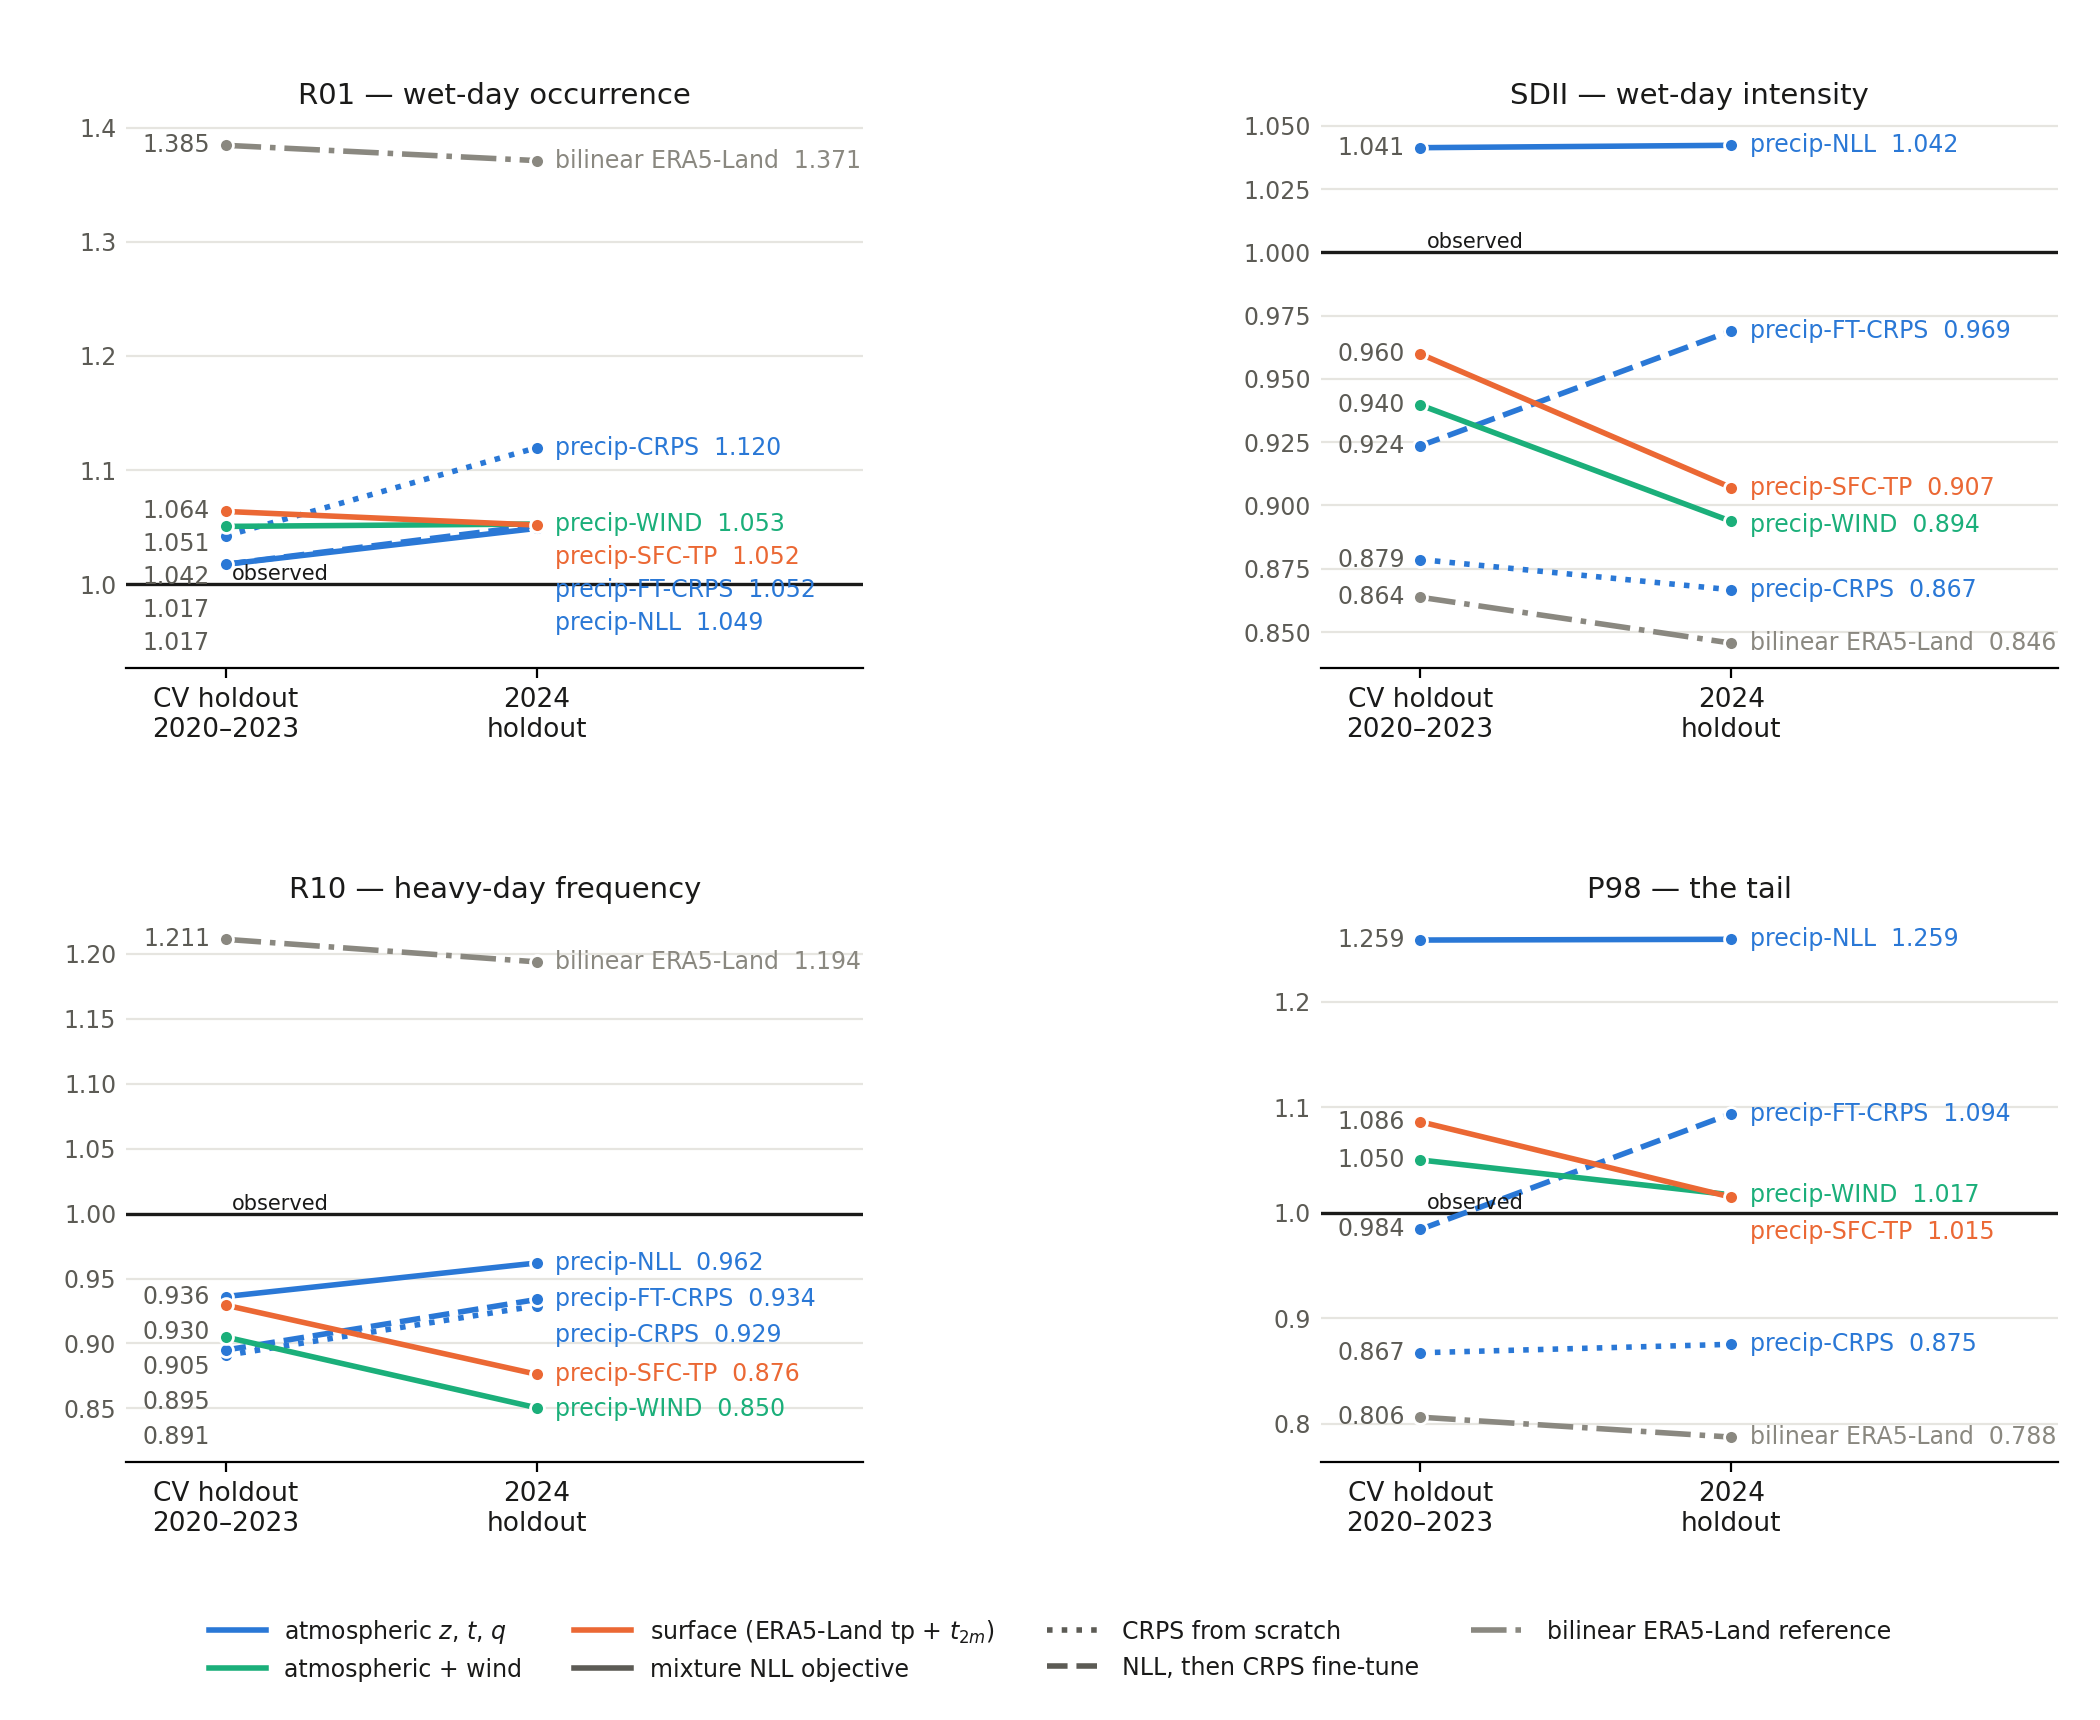
\includegraphics[width=\textwidth]{images/precip_regime_slope_indices.png}
\caption[The four physical precipitation indices]{The four physical precipitation indices of
\tref{tab:app-metrics-overview} from the CV holdout to the unseen year, on the conventions of
\fref{fig:single-precip-slope}: occurrence (R01), typical intensity (SDII), heavy-day frequency
(R10) and the tail (P98). Every panel is a predicted-over-observed ratio.}
\label{fig:precip-indices}
\end{figure}
\fref{fig:precip-indices} carries occurrence and intensity into the heavy categories, adding the heavy-day frequency R10 and the tail P98 to the two indices already seen. Each is a predicted-over-observed ratio, so one is a perfect match in every panel. R01 makes the occurrence gap quantitative, the reference overshooting the observed wet-day frequency by $+38\,\%$ where no run departs by more than $+7\,\%$ on the CV holdout, and heavy-day frequency behaves the same way, the reference overshooting R10 by $+21\,\%$ while every run undershoots it by between $6$ and $11\,\%$. The extreme tail is the one index where the reference beats a run: it undershoots P98 by $-19\,\%$, \texttt{precip-NLL} overshoots it by $+26\,\%$. On the unseen year the reference behaves much as it does on the training span, and so do \texttt{precip-SFC-TP} and \texttt{precip-WIND}; the three objective variants improve on R10 while \texttt{precip-FT-CRPS} drifts back towards \texttt{precip-NLL} in SDII and P98.


Neither the raw measures nor the indices provide a clear response to which model performs best: 
different runs score best on different indices, and on two of them, MAE and rank correlation, the reference beats every run.

\subsection{Skill by Intensity Category}\label{subsec:single-precip-categories}

Precipitation is a harder downscaling target than temperature, and the reason lies in how the
observations are distributed rather than in the models. Over the CV holdout $52\,\%$ of point-days
are dry and a further $36\,\%$ stay below $10\,\mathrm{mm}$, while the two heaviest categories
together account for under $1\,\%$. Any score pooled over that distribution is therefore decided by
days on which little happens, whereas the days a downscaling product is wanted for sit in a tail
thin enough that the estimates there rest on few events and carry a correspondingly wide spread.
In \fref{fig:single-precip-categories} the brier scores for the different intensity categories are reported.

\begin{figure}[H]
\centering
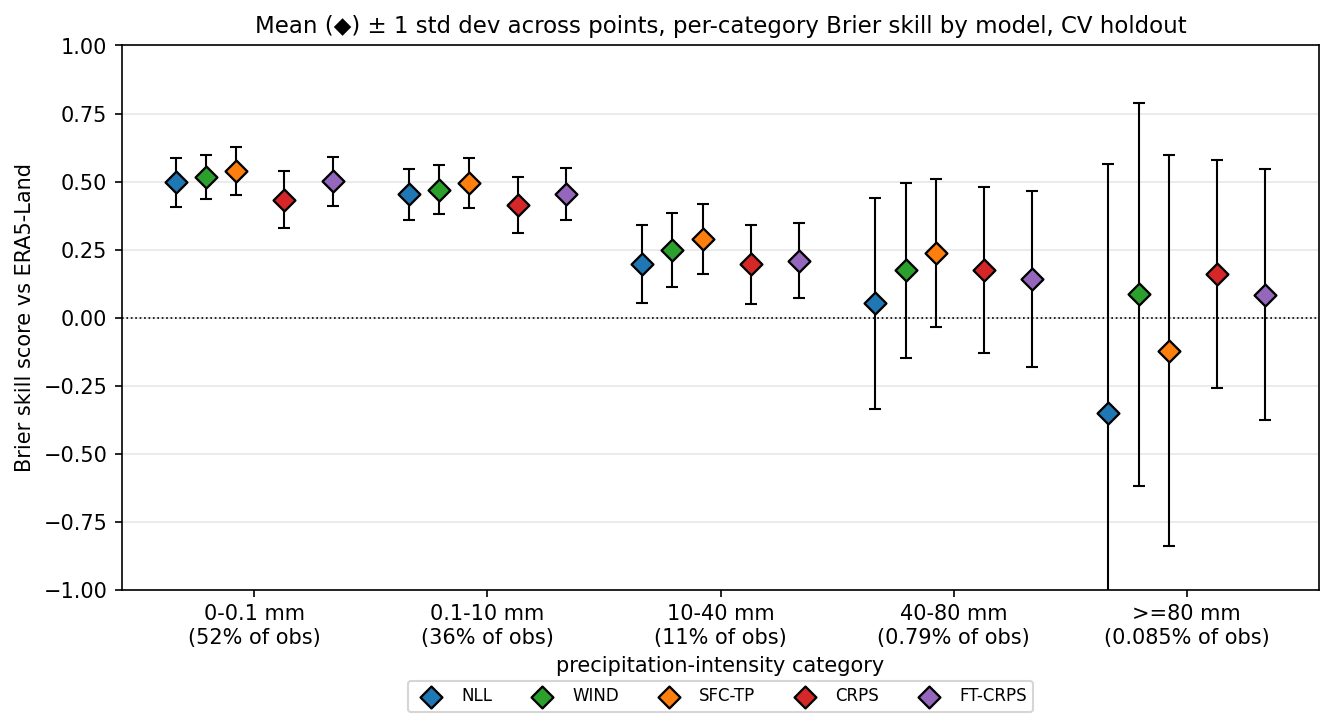
\includegraphics[width=\textwidth]{images/results/precip__bss_category_comparison__precip_processing_comparison__ALL.png}
\caption[Brier skill by intensity category]{Brier skill score against the bilinear ERA5-Land
reference, by intensity category evaluated on CV holdout. Positive means
the run places that category's probability better than the reference. Every grid point first gets its own
Brier skill score then we average over the points. The diamond is then the mean of those per-point skills over the domain and the
whisker their $\pm1$ standard deviation. The whisker is therefore a spatial spread, not a standard
error.}
\label{fig:single-precip-categories}
\end{figure}

Read by intensity category, three things follow. Almost all of the pooled skill is earned in the two categories that carry $88\,\%$ of point-days, where all five models sit close together between $+0.41$ and $+0.54$ and clearly beat the reference. Skill then falls monotonically with intensity, and the estimate loses significance as it goes: by $\geq 80\,\mathrm{mm}$ the spread across grid points is several times the mean for every model. The ordering shifts in the two heaviest categories, most of all in the last. \texttt{precip-SFC-TP}, first almost everywhere else, and \texttt{precip-NLL} both fail there, while \texttt{precip-CRPS} holds the best tail on both mean and spread and \texttt{precip-FT-CRPS} is the best compromise, keeping nearly all of \texttt{precip-WIND}'s skill in the frequent categories and nearly all of \texttt{precip-CRPS}'s tail robustness. Because RPSS weights by frequency and that category is $0.085\,\%$ of point-days, none of it registers in \tref{tab:single-precip-selection}: reading the two together is what separates a model that is uniformly good from one that is good where the days are.


\fref{fig:single-precip-spatial-categories} visualises this comparison for the two best balanced models \texttt{precip-SFC-TP} and \texttt{precip-FT-CRPS}. The observed frequencies are put next to the reference and the model frequencies and the skill column presents the spatial skill distribution.
\begin{figure}[p]
\centering
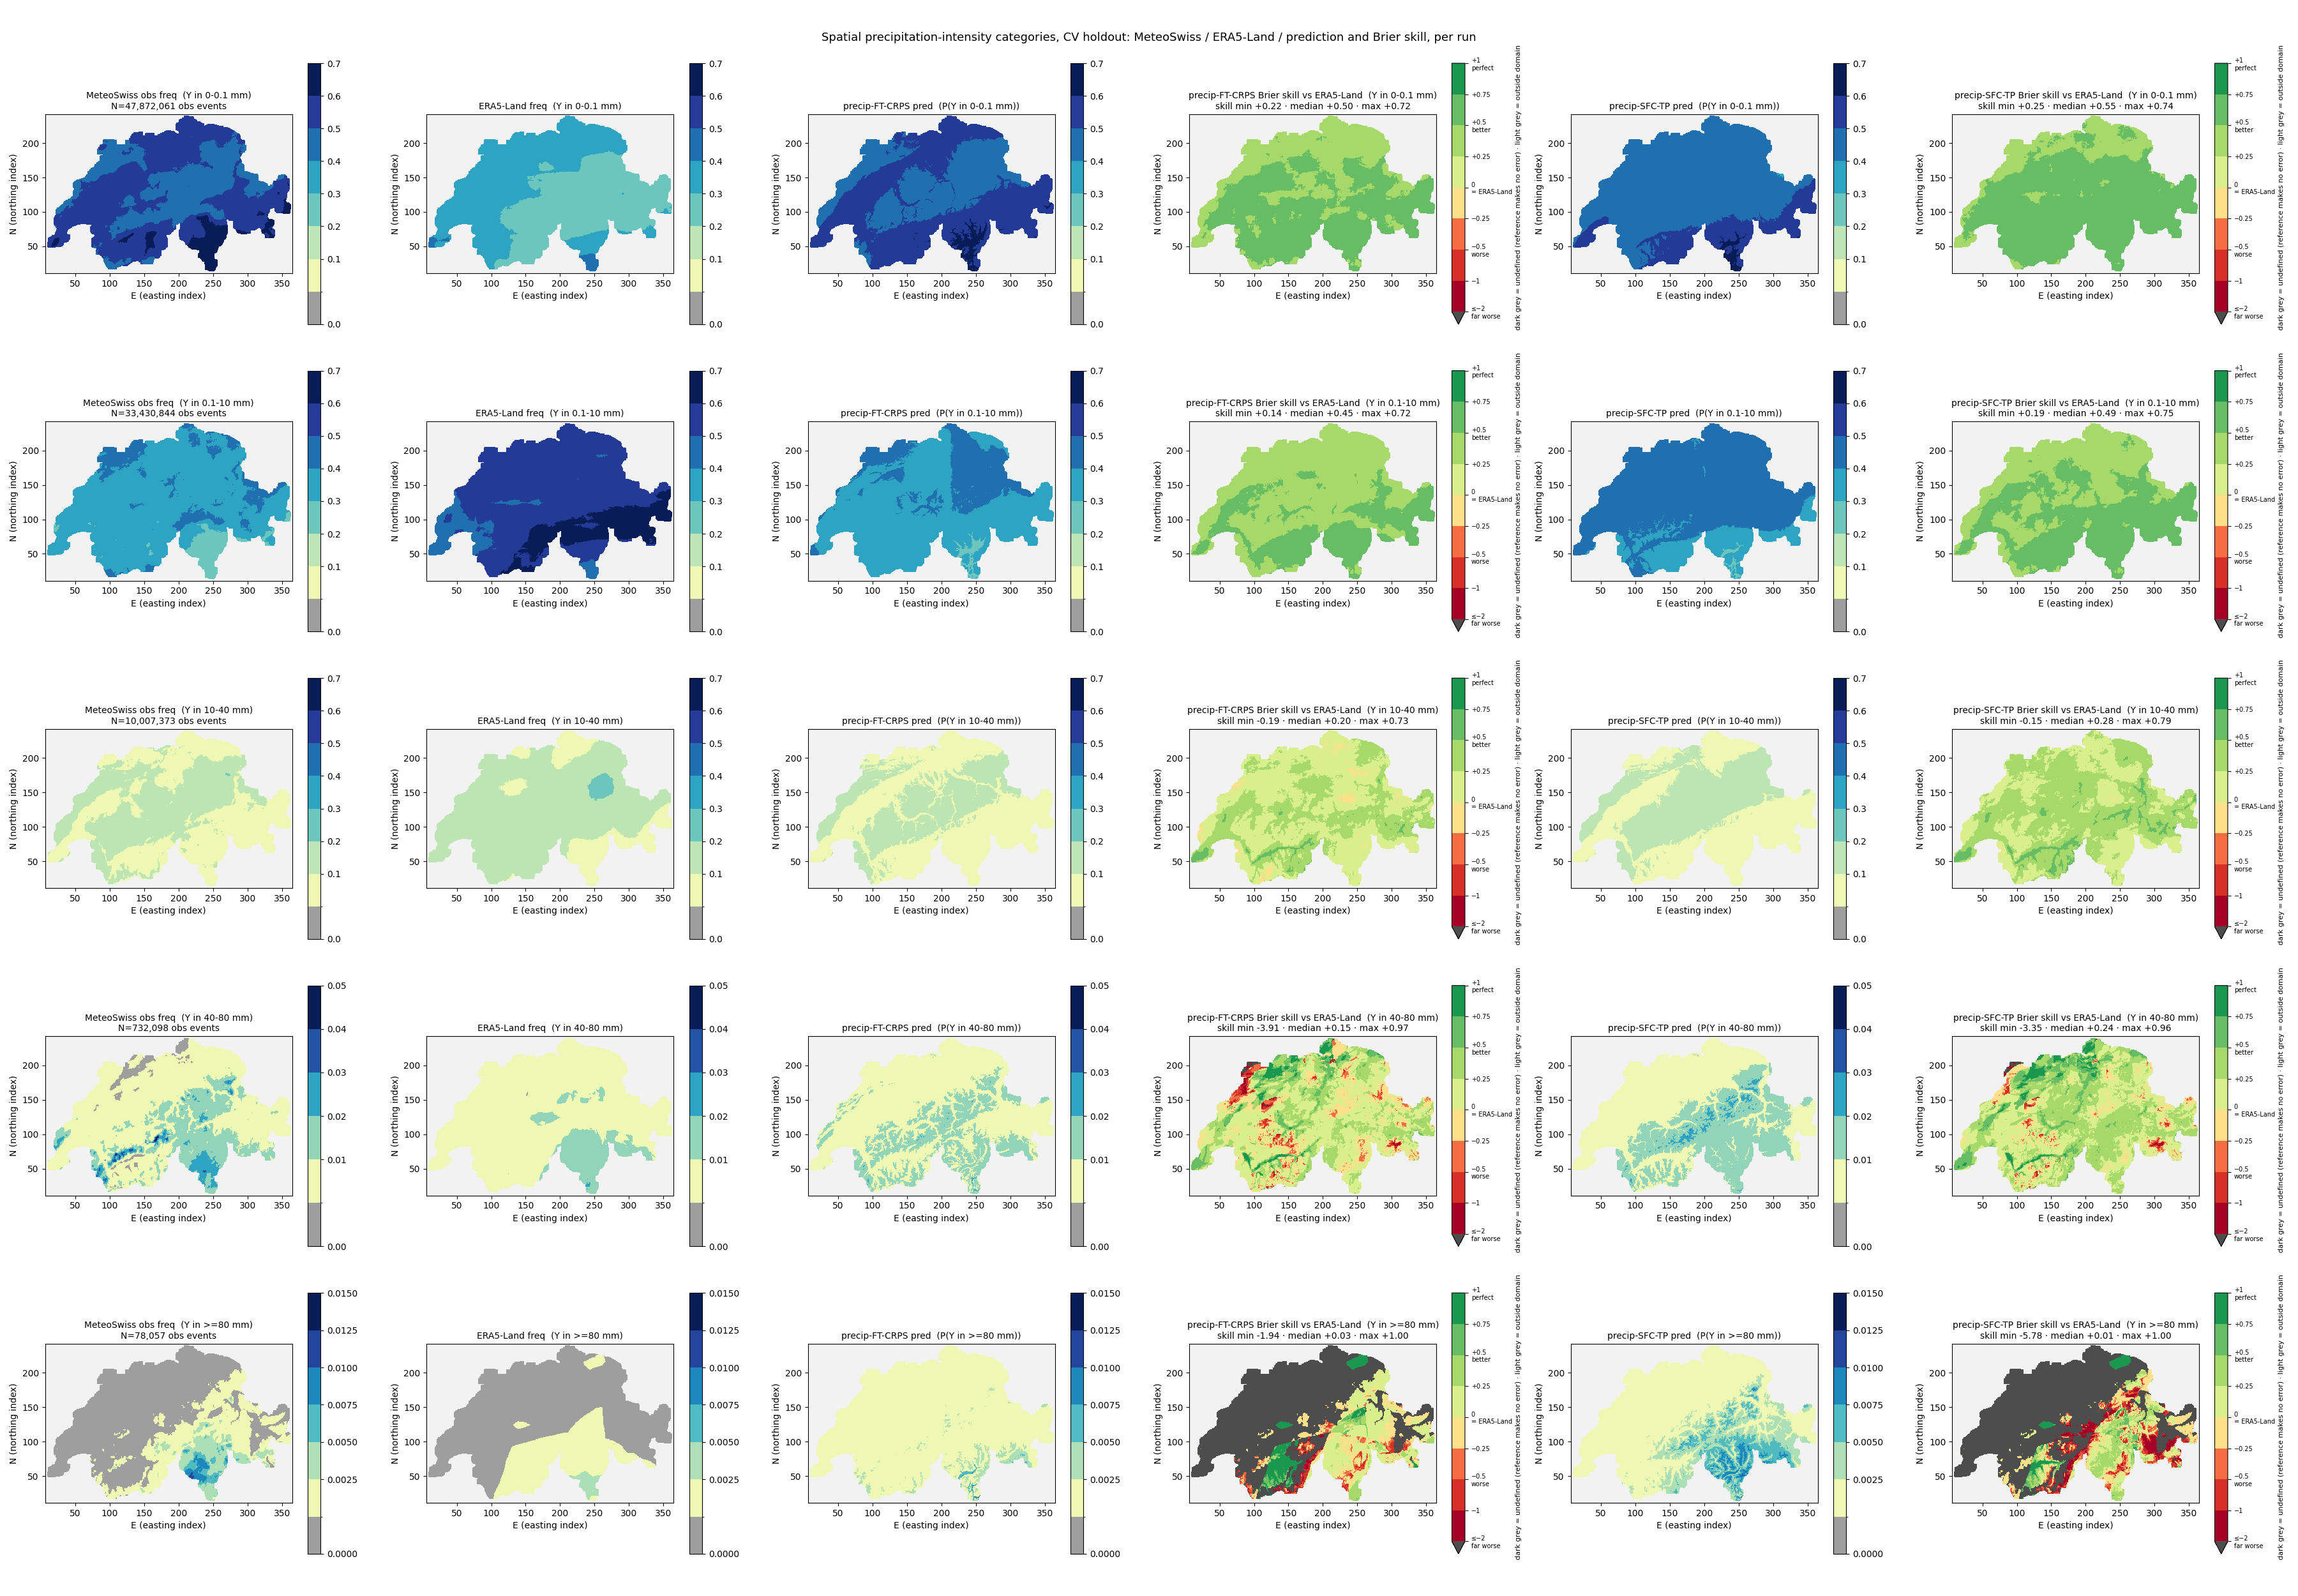
\includegraphics[angle=90,origin=c,width=\linewidth,height=0.92\textheight,keepaspectratio]{images/results/precip__category_spatial_pair__precip_processing_comparison__ALL.png}
\caption[Spatial distribution of Categorical Brier Skill score]{Spatial distribution of Brier skill by rain category for fine-tuned and the surface run. Rows Intensity categories, Columns from left to right observed frequency, reference frequency, FT-CRPS frequency, FT-CRPS Skill, SFC frequency, SFC skill.}
\label{fig:single-precip-spatial-categories}
\end{figure}


In the first three categories (dry days $<0.1\,\mathrm{mm}$, drizzle $0.1$--$10\,\mathrm{mm}$ and
ordinary rain days $10$--$40\,\mathrm{mm}$) both models perform well, and \texttt{precip-SFC-TP} is
slightly ahead on the numbers, its median skill exceeding that of \texttt{precip-FT-CRPS}. The spatial fields separate them more than the numbers do.
\texttt{precip-FT-CRPS} resolves the terrain, its frequency bands following the Alpine ridges and
valleys, whereas
\texttt{precip-SFC-TP} stays closer to the reference's own spatial distribution.

The two heavy categories behave differently from each other, and only the heaviest separates the
runs significantly. Between $40$ and $80\,\mathrm{mm}$ \texttt{precip-SFC-TP} is still ahead. Above $80\,\mathrm{mm}$ the ordering
reverses: the two median skills over grid points are effectively tied at $+0.01$ and $+0.03$, but the
surface run's worst point falls to $-5.78$ where the fine-tuned run holds $-1.94$. 
\texttt{precip-SFC-TP} predicts extreme-event frequencies at roughly the observed magnitude but
spreads them over large areas that never observe such events, so where it is wrong it is wrong by a
wide margin; \texttt{precip-FT-CRPS} stays conservative and keeps its losses bounded. Due to the sparsity of observed points in this category such patches are
difficult to avoid. No terrain feature explains their placement; the error along the Jura ridge is
more likely a domain-edge effect, since the loss is formed only at target points inside Switzerland
(\sref{objective}) and border regions are therefore constrained from one side only.

This confirms the reading of \fref{fig:single-precip-categories}: \texttt{precip-FT-CRPS} combines
acceptable skill in the frequent categories with a bounded worst case in the tail, while
\texttt{precip-SFC-TP} is the better model on average and the worse one when it fails. Which of the
two to prefer is therefore an application decision, whether the use case is dominated by the
categories that carry the point-days, or by the cost of a large error in a rare extreme event. The same maps for the three remaining runs are given in
\sref{sec:app-precip-category-spatial}.

\subsection{Feature Importance}\label{subsec:single-precip-fi}
The feature importance study shows clear signs that the atmospheric configurations spread
their reliance across the meteorological channel groups rather than leaning on any single one
(\fref{fig:single-precip-fi}).

Compared to the temperature model in \sref{sec:single-temperature} the specific humidity rather than the temperature dominates the variable panel. The dominance of humidity is significant but the geopotential and the temperature contribute substantial shares ($z \approx 1$ to $t \approx 3$--$4$ to $q \approx 8$--$9$). The model thus balances the three input channel groups rather than overfitting on a single one while the surface run is completely dominated by the tp channel.

Importance is spread over every pressure level and every hour, where the temperature models concentrate on $1000$ and $925\,\mathrm{hPa}$ and the midday hours. The largest single share sits at $500\,\mathrm{hPa}$ in every run, in the mid-troposphere rather than near the ground, and the $06$~UTC snapshot leads the hours in all but \texttt{precip-WIND}, where $18$~UTC takes over.

Wind and scaffold channels are the least important, with the seasonal encoding contributing very little to the result.
\begin{figure}[H]
\centering
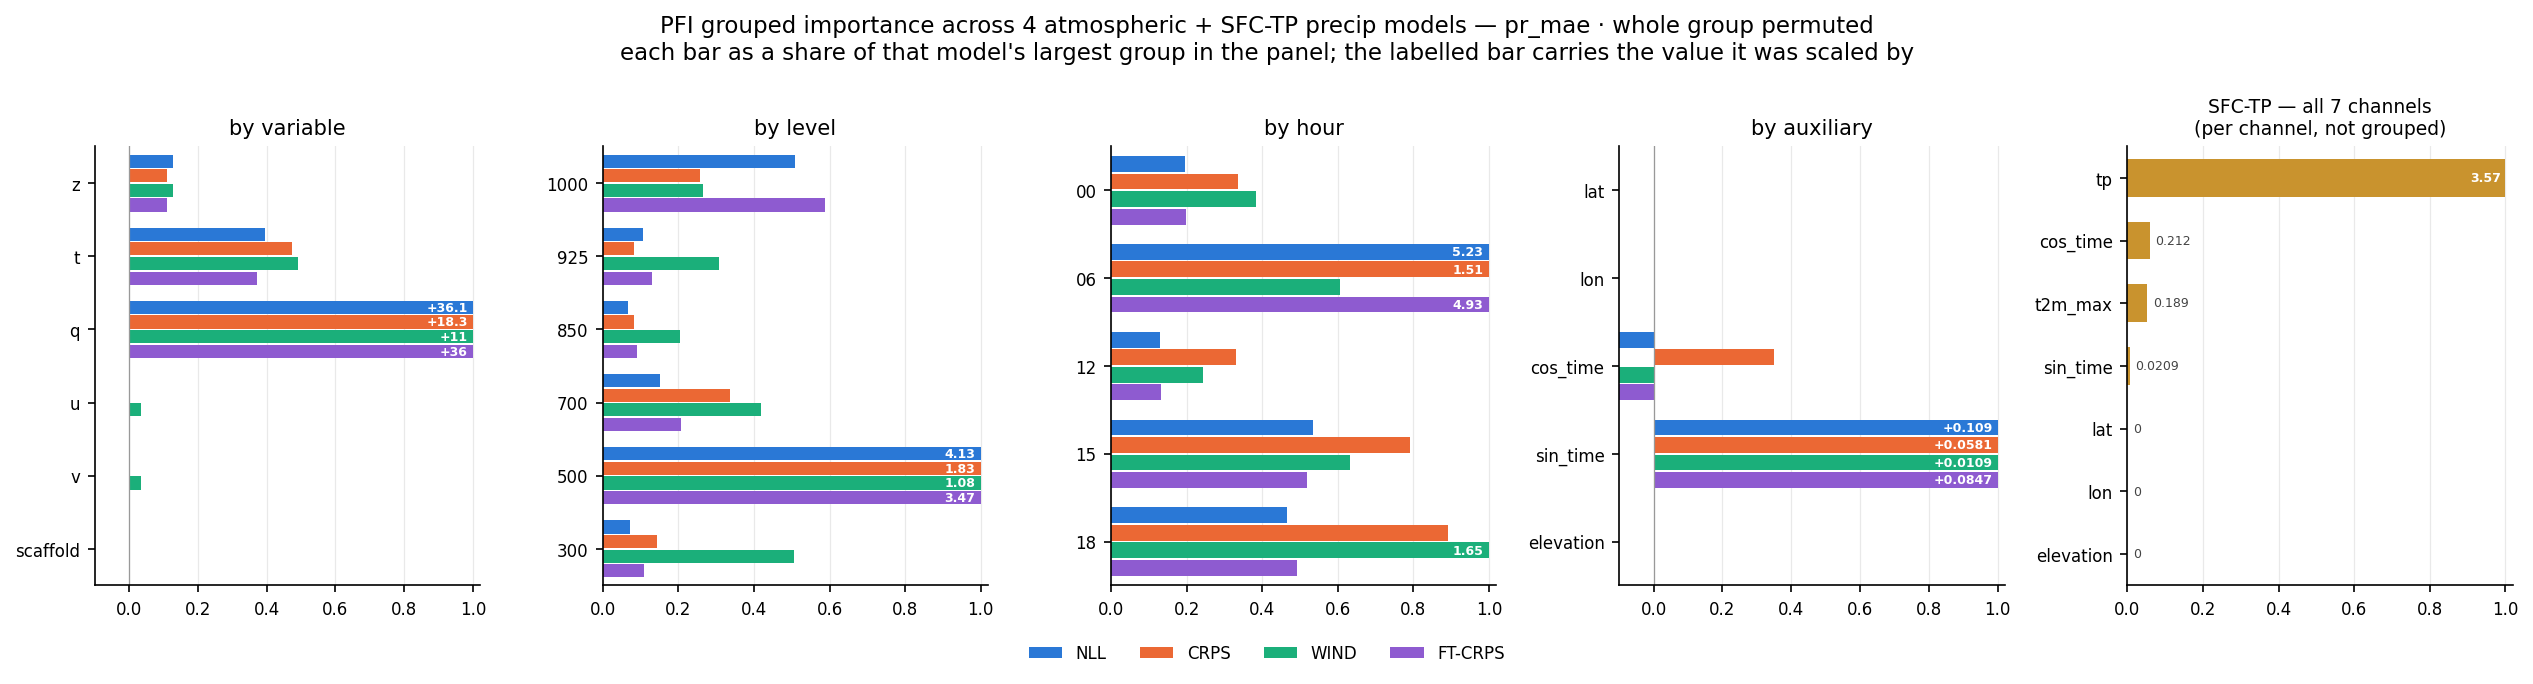
\includegraphics[width=\textwidth]{images/results/precip__fi_group_importance_pfi_2024__precip_processing_comparison__ALL.png}
\caption[Grouped permutation importance across the precipitation runs]{Grouped permutation
importance for the four atmospheric precipitation runs, on the 2024
holdout. Each model in the atmospheric runs is normalised by its peak contribution within each of the groups, to highlight relative importances. The normalisation constant is provided for each model in the full-length bar. \texttt{precip-SFC-TP} has no group permutation and is therefore represented independently. A bar
at or below zero means permuting that group changed the error by less than the noise of the estimate
itself, so it records no measurable contribution rather than a harmful one; the negative side of the
axis is cut short for that reason, and a bar reaching the cut is not a large negative.}
\label{fig:single-precip-fi}
\end{figure}


\subsection{Calibration}\label{subsec:single-precip-calibration}
Calibration is assessed with the probability integral transform of \fref{fig:single-precip-pit}, and
it enters the selection as a check rather than as a criterion.
\begin{figure}[H]
\centering
\subfloat[\texttt{precip-SFC-TP}]{%
  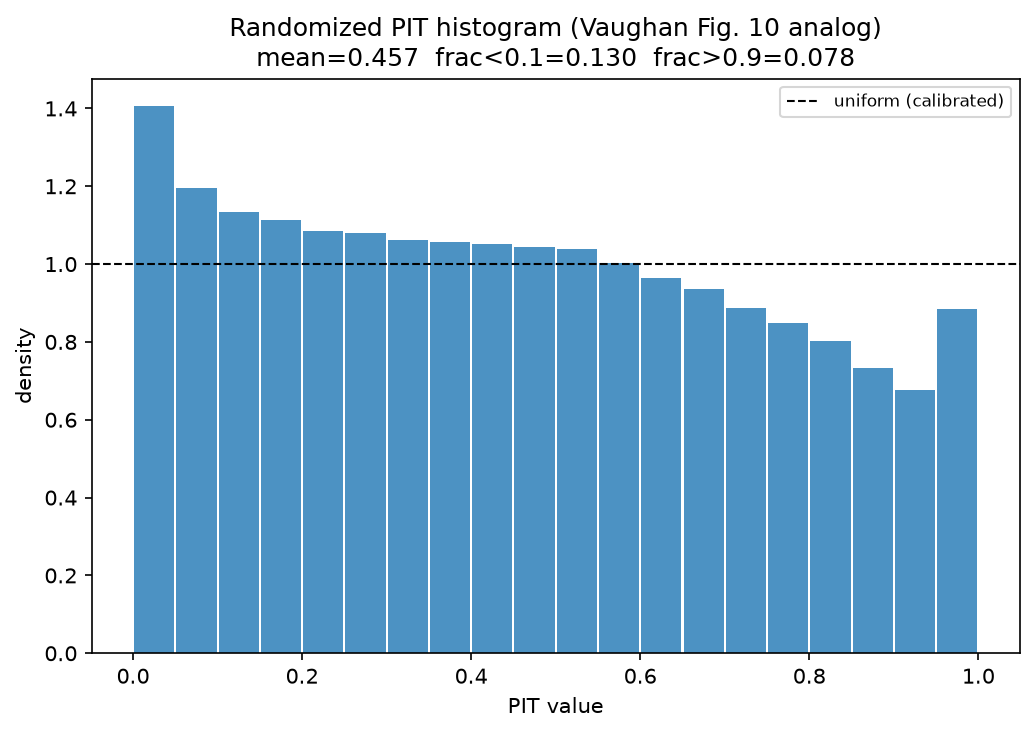
\includegraphics[width=0.49\textwidth]{images/results/precip__pit_histogram__eval_cv__clean_solo_precip_sfctp.png}}
\hfill
\subfloat[\texttt{precip-FT-CRPS}]{%
  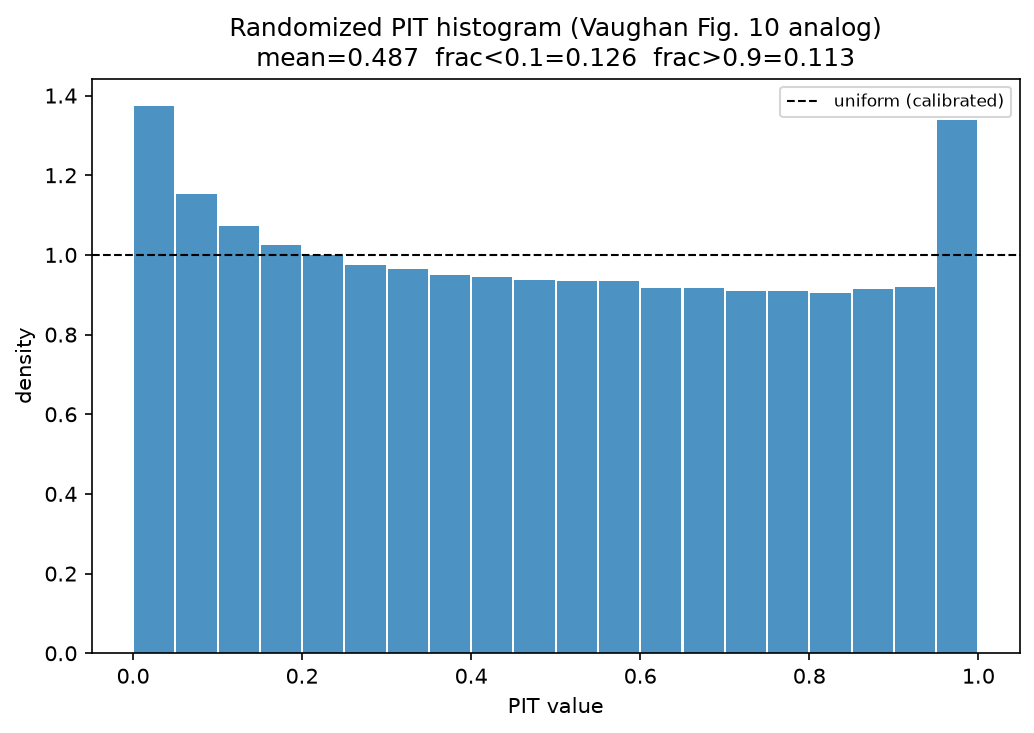
\includegraphics[width=0.49\textwidth]{images/results/precip__pit_histogram__eval_cv__clean_solo_precip_ftcrps.png}}
\caption[PIT histograms for the two selected runs]{Probability integral transform for the two
selected runs on the CV holdout, with the randomisation at the discrete point mass described in
\sref{subsec:app-skill-precip}. A calibrated forecast gives a flat histogram; a tilt towards low
values means too much probability is placed below the value that occurred.}
\label{fig:single-precip-pit}
\end{figure}

Every run places somewhat too much probability below the value that occurred. On the CV holdout the
PIT means of both selected models sit below the ideal $0.5$, \texttt{precip-FT-CRPS} at $0.487$ and
\texttt{precip-SFC-TP} at $0.457$. The PITs for the other models are reported in \tref{tab:single-precip-selection}.
\texttt{precip-SFC-TP} leans, carrying significant mass below $0.1$ and missing mass above 0.6,
whereas \texttt{precip-FT-CRPS} is nearly symmetric and departs from the ideal flat
 distribution as a shallow U rather than as a lean. Its leading PIT mean is therefore a near-balance of the two
ends rather than an absence of miscalibration.

The miscalibration is there in both models, but it is modest and of the same kind, a tilt of the
distribution rather than a collapse of the spread, and it points the same way for every run, so it
reorders none of the comparisons made above. Calibration enters the
model evaluation as a check  rather than a selection criterion and all models present acceptable calibration.

\FloatBarrier
\subsection{Model Selection}\label{subsec:single-precip-selection}

Unlike temperature (\sref{subsec:single-tmax-geography}), no single precipitation run leads on every
axis, so the choice here has to be argued rather than read off one figure.
\tref{tab:single-precip-selection} collects the evidence: the two skill scores against the bilinear
ERA5-Land reference, the Brier skill of \fref{fig:single-precip-categories} resolved
into its five intensity bands, the signed P98 tail bias and the PIT mean of
\sref{subsec:single-precip-calibration}, all on the CV holdout.

The aim in this work is to find a model that performs well and is robust. The winner is not clear. From feature importance \sref{subsec:single-precip-fi} we learn that the atmospheric models do appear to rely on the complexity of the diurnal cycle of the different input channels rather than overfitting on a single input channel. While the SFC model performs best in most
metrics, it fails in the extreme tail, where it is one of only two runs with a negative Brier skill
($-0.121$), and its lead rests almost entirely on the ERA5-Land total precipitation channel.
\texttt{precip-FT-CRPS} wins no column, but it is positive in all five bands, worst in none and the
closest to a uniform PIT. \texttt{precip-WIND} scores very similarly. However, as we saw for
temperature, its richer input probably needs a longer training budget to reach its potential.
\texttt{precip-NLL} and \texttt{precip-CRPS} fall off in performance: the first is worst in both heavy bands
and on the tail bias, the second is the weakest of the five in the three lightest bands, which hold nearly all of the
days.

We therefore keep two runs, one per input family. \texttt{precip-SFC-TP} is the choice wherever a
simple model is enough and the tail is not the target, \texttt{precip-FT-CRPS} the robust choice based on
atmospheric input.

\begin{table}[H]
\centering
\caption[Model-selection scorecard, all five precipitation runs]{The model-selection scorecard, on
the CV holdout. RPSS (\eref{eq:rpss}) and MAE skill (\eref{eq:mae-skill}) are both scored
against the shared bilinear ERA5-Land reference. The five BSS columns give the mean and standard
deviation, over the domain, of the per-point Brier skill of \fref{fig:single-precip-categories}, one column per intensity category.
The standard deviation is the spread across grid points, not an
uncertainty on the mean. P98 from \fref{fig:precip-indices},
positive meaning an overshot tail; PIT mean is from \sref{subsec:single-precip-calibration}, ideal
$0.5$. Green shades the best and red the worst run in each column, and the heavy rules pick out
\texttt{precip-FT-CRPS}, the atmospheric selected run. }
\label{tab:single-precip-selection}
\scriptsize
\setlength{\tabcolsep}{1.5pt}
\renewcommand{\arraystretch}{1.25}
\begin{tabular}{|>{\raggedright\arraybackslash}p{2.1cm}|>{\centering\arraybackslash}p{0.9cm}|>{\centering\arraybackslash}p{0.9cm}|>{\centering\arraybackslash}p{1.6cm}|>{\centering\arraybackslash}p{1.6cm}|>{\centering\arraybackslash}p{1.6cm}|>{\centering\arraybackslash}p{1.6cm}|>{\centering\arraybackslash}p{1.6cm}|>{\centering\arraybackslash}p{0.9cm}|>{\centering\arraybackslash}p{0.85cm}|}
\hline
\textbf{Run} & \textbf{RPSS} & \textbf{MAE} \newline \textbf{skill} &
\textbf{BSS dry} \newline \textbf{0--0.1} & \textbf{BSS weak} \newline \textbf{0.1--10} &
\textbf{BSS mod.} \newline \textbf{10--40} &
\textbf{BSS heavy} \newline \textbf{40--80} & \textbf{BSS extr.} \newline $\mathbf{\geq 80}$ &
\textbf{P98} \newline \textbf{(mm)} & \textbf{PIT} \newline \textbf{mean} \\
\hline
\texttt{precip-NLL} & $0.408$ & \cellcolor{red!12}$-0.234$ & $0.497 \pm 0.09$ & $0.453 \pm 0.09$ &
$0.198 \pm 0.14$ &
\cellcolor{red!12}$0.052 \pm 0.39$ & \cellcolor{red!12}$-0.350 \pm 0.91$ &
\cellcolor{red!12}$+11.15$ & $0.469$ \\
\hline
\texttt{precip-CRPS} & \cellcolor{red!12}$0.366$ & $-0.187$ & \cellcolor{red!12}$0.433 \pm 0.11$ &
\cellcolor{red!12}$0.415 \pm 0.10$ & \cellcolor{red!12}$0.195 \pm 0.14$ & $0.175 \pm 0.31$ & \cellcolor{green!12}$0.161 \pm 0.42$ &
$-5.71$ & \cellcolor{red!12}$0.418$ \\
\noalign{\hrule height 1.1pt}
\texttt{precip-FT-CRPS} & $0.416$ & $-0.145$ & $0.501 \pm 0.09$ & $0.454 \pm 0.09$ &
$0.209 \pm 0.14$ &
$0.140 \pm 0.32$ & $0.085 \pm 0.46$ & \cellcolor{green!12}$-0.68$ &
\cellcolor{green!12}$0.487$ \\
\noalign{\hrule height 1.1pt}
\texttt{precip-WIND} & $0.443$ & $-0.092$ & $0.518 \pm 0.08$ & $0.470 \pm 0.09$ &
$0.247 \pm 0.14$ &
$0.173 \pm 0.32$ & $0.086 \pm 0.70$ & $+2.16$ & $0.463$ \\
\hline
\texttt{precip-SFC-TP} & \cellcolor{green!12}$0.473$ & \cellcolor{green!12}$-0.032$ &
\cellcolor{green!12}$0.538 \pm 0.09$ & \cellcolor{green!12}$0.494 \pm 0.09$ &
\cellcolor{green!12}$0.288 \pm 0.13$ &
\cellcolor{green!12}$0.238 \pm 0.27$ & $-0.121 \pm 0.72$ & $+3.73$ & $0.457$ \\
\hline
\end{tabular}
\end{table}


Both selections hold up on the unseen year. The RPSS ordering of \fref{fig:single-precip-slope-skill}
is reproduced exactly in 2024, and both runs give up about $0.065$, as do the other three, so the loss
is shared rather than specific to either. Their MAE rises by $0.3$ and $0.45\,\mathrm{mm}$
(\fref{fig:single-precip-slope}), but the bilinear reference worsens by $0.28\,\mathrm{mm}$ in step,
so the distance to it barely moves and the MAE skill slips by only $0.01$ and $0.05$: 2024 is a
harder year rather than a year the models fail on. The indices of \fref{fig:precip-indices} agree,
both runs holding wet-day occurrence within a few percent of observed under either regime. 





\subsection{Discussion}\label{subsec:single-precip-discussion}



Two results of this section are worth separating from the model ranking. The first is that pointwise
error and distributional skill disagree in sign: no run beats bilinear interpolation in millimetres,
yet every run beats it by a wide margin on the five-category RPSS and on occurrence and intensity.
This is the behaviour the literature predicts. A smoothed coarse field is hard to beat on a squared
or absolute error while being wrong about the shape of the distribution, which is why the reference
calls wet days $38\,\%$ too often where the runs stay within a few per cent. The Bernoulli--Gamma
head is what buys that correction, as \textcite{cannon2008berngamma} report for density networks and
\textcite{vaughan2022convcnp} adopt for the same reason; the indices used here are theirs, and they
are used precisely because a pointwise score would hide the improvement. Their European,
station-based evaluation is not directly comparable to a Swiss gridded target, so no number is set
against theirs. The feature importance adds the interpretability side of the same point: the
atmospheric runs distribute their reliance across humidity, temperature and geopotential rather than
onto one channel, which is the meteorological rather than geographical reliance. \textcite{rampal2022interpretable} report the same for a grid-to-grid network over the New Zealand Southern Alps, read off saliency maps rather than permutation importance, so the conclusion now holds across two mountainous domains, two model geometries and two attribution methods.

The second is that the issue of extreme tail remains unsolved. The tail reversal of
\sref{subsec:single-precip-categories} is a CV-holdout result only: on 2024 the heaviest category is
negative for \emph{every} run, from \texttt{precip-SFC-TP} at $-0.05$ to \texttt{precip-NLL} at
$-0.21$, so \texttt{precip-CRPS}'s advantage there should not be carried over. A parametric
per-point head, whatever objective trains it, models each target point independently and has little
to work with where events are this rare. Generative and autoregressive approaches
\cite{harris2022generative, mardani2025corrdiff, bruinsma2023arcnp} address exactly this regime, at
the cost of the calibration that the present head gives directly.



\subsection{Conclusion}\label{subsec:single-precip-conclusion}

Two runs are carried forward: \texttt{precip-SFC-TP} where a simple surface model suffices, and
\texttt{precip-FT-CRPS} where robustness across the intensity range matters. Both correct the
occurrence and intensity errors of the coarse field, and both do so by a wide margin: their RPSS
against the bilinear ERA5-Land reference is $+0.47$ and $+0.42$ on the CV holdout and $+0.41$ and
$+0.35$ on the unseen year, a reduction of the ranked probability error of a third to a half in
either regime. Neither, however, improves on plain interpolation in millimetres. The heaviest rain remains the limit of what
this architecture and likelihood can deliver. 

